\documentclass{plt}

\newcommand{\tocbreak}{\addtocontents{toc}{\vfill\protect\pagebreak\null\medskip}}

% Make | a mathrel symbol: improves alternation (a | b) spacing
\mathcode`\|="326A

\tikzset{double distance=1pt,>=latex}

\tikzset{
  parsetree/.style={
    level distance=2pc,
    sibling distance=1.8pc,
    every node/.style={fill=white},
    every path/.style={thick},
    baseline=(current bounding box.west)
  },
  connecting lines/.style={remember picture, overlay,
    every path/.style={->,red,opacity=0.5,line width=2pt}},
  byte/.style={fill=gray,minimum height=16pt,minimum width=20pt,text=white},
  hbyte/.style={fill=darkred,minimum height=16pt,minimum width=20pt,text=white},
  bytes/.style={matrix of nodes/.style={
           execute at begin cell=\node\bgroup,
           execute at end cell=\egroup;,
           execute at empty cell={\node [byte] {};}},
           matrix of nodes,
           every node/.style=hbyte},
  free/.style={draw,minimum height=16pt},
  used/.style={draw,fill=gray,minimum height=16pt},
}

% Work around a tikz bug
\makeatletter
\def\pgf@test{}
\makeatother

%\newcommand{\hlt}[1]{\textcolor{red}{#1}}
\newcommand{\lab}[3]{\tikz{\useasboundingbox (0,0);
    \node [draw, anchor=west,fill=black!10,rectangle callout,
      callout absolute pointer={(1pt,3pt)}]
  at (#1,#2) {\rmfamily{#3}}; 
}}

\def\hlta<#1>{\alt<#1>{\color{black}}{\color{gray}}}

\lstdefinelanguage{cbnf}{%
  columns=flexible,%
  basicstyle={\footnotesize},%
  identifierstyle={\sffamily\itshape},%
  comment=[l]{\#},%
  commentstyle={\color{red}},%
  keywords={void,char,short,int,long,float,double,signed,unsigned,struct,%
    typedef,extern,static,enum,extern,auto,union,register,enum,const,volatile},%
  alsoletter={-},%
  literate={_opt}{$_{\textit{opt}}$}4,%
}

\newcommand{\rnode}[2]{\tikz[baseline,remember picture]
  \node [anchor=text,inner sep=0pt] (#1) {#2};}

\newcommand{\framednode}[2]{\tikz[baseline,remember picture]
  \node [anchor=text,draw] (#1) {#2};}

% For drawing arithmetic parse trees

\def\plus#1#2{node {\texttt{+}} child {#1} child {#2}}
\def\minus#1#2{node {\texttt{-}} child {#1} child {#2}}
\def\mult#1#2{node {\texttt{*}} child {#1} child {#2}}
\def\lit#1{node {#1}}

\tikzfading[name=fade down,
  top color=transparent!0,
  bottom color=transparent!100]

\tikzfading[name=fade up,
  bottom color=transparent!0,
  top color=transparent!100]

\newcommand{\pac}{\cdot}

\title{Review for the Final Exam}
\author{Stephen A. Edwards}
\institute{Columbia University}
\date{Fall 2018}
\titlegraphic{\includegraphics[width=0.5\textwidth]{dont-panic.jpg}}

\begin{document}

\frame{\titlepage}

\begin{frame}[allowframebreaks]{Table of Contents}
\parskip=1pt plus 4pt
\tableofcontents
\end{frame}

\section{The Final Exam}

\begin{frame}{The Final}

75 minutes

Closed book

One double-sided sheet of notes of your own devising

Comprehensive: Anything discussed in class is fair game, including
things from before the midterm

Little, if any, programming

Details of O'Caml/C/C++/Java/Prolog syntax not required

Broad knowledge of languages discussed

\end{frame}

\section{Structure of a Compiler}

\begin{frame}[fragile=singleslide]
  \frametitle{Compiling a Simple Program}

\begin{C}
int gcd(int a, int b)
{
  while (a != b) {
    if (a > b) a -= b;
    else b -= a;
  }
  return a;
}
\end{C}

\end{frame}

\newsavebox{\gcdbox}
\begin{lrbox}{\gcdbox}
\begin{minipage}{0.4\textwidth}
\begin{C}
int gcd(int a, int b)
{
  while (a != b) {
    if (a > b) a -= b;
    else b -= a;
  }
  return a;
}
\end{C}
\end{minipage}
\end{lrbox}

%%%%%%%%%%%%%%%%%%%%%%%%%%%%%%

\begin{frame}[fragile=singleslide]
  \frametitle{What the Compiler Sees}

\usebox{\gcdbox}

\begin{verbatim}
i  n  t sp  g  c  d  (  i  n  t sp  a  , sp  i
n  t sp  b  ) nl  { nl sp sp  w  h  i  l  e sp
(  a sp  !  = sp  b  ) sp  { nl sp sp sp sp  i
f sp  (  a sp  > sp  b  ) sp  a sp  -  = sp  b
; nl sp sp sp sp  e  l  s  e sp  b sp  -  = sp
a  ; nl sp sp  } nl sp sp  r  e  t  u  r  n sp
a  ; nl  } nl
\end{verbatim}

Text file is a sequence of characters

\end{frame}

%%%%%%%%%%%%%%%%%%%%%%%%%%%%%%

\begin{frame}[fragile=singleslide]
  \frametitle{Lexical Analysis Gives Tokens}

\usebox{\gcdbox}\hfill
\includegraphics[width=0.45\textwidth]{subway-tokens.jpg}

\newbox\mystrutbox
\setbox\mystrutbox=\hbox{\vrule height7.5pt depth2.5pt width0pt}
\def\strut{\relax\ifmmode\copy\mystrutbox\else\unhcopy\mystrutbox\fi}

\def\frame #1 #2 #3 #4 #5 #6 #7 #8
{\framebox{\strut #1} 
\framebox{\strut #2} 
\framebox{\strut #3} 
\framebox{\strut #4}
\framebox{\strut #5} 
\framebox{\strut #6} 
\framebox{\strut #7} 
\framebox{\strut #8}
}

{\ttfamily
\frame int gcd ( int a , int b
\frame ) \{ while ( a != b )
\frame \{ if ( a $>$ b ) a
\frame -= b ; else b -= a ;
\framebox{\strut\}} \framebox{\strut return} \framebox{\strut a}
\framebox{\strut ;} \framebox{\strut \}}
}

A stream of tokens.  Whitespace, comments removed.

\end{frame}

\newcommand{\id}[1]{
  node [fill=white] {#1}
}

\newcommand{\theast}{
  \node {func} [level distance=2pc,
    level 1/.style={sibling distance=3.5pc},
    level 2/.style={sibling distance=4.5pc},
    level 3/.style={sibling distance=2.5pc},
    level 4/.style={sibling distance=2.5pc},
    level 5/.style={sibling distance=1.5pc},
  ]
  child {node {int}}
  child {node {gcd}}
  child {node {args}
    child {node {arg}
      child {node {int}}
      child {\id a}}
    child {node {arg}
      child {node {int}}
      child {\id b}}
  }
  child [missing]
  child [missing]
  child {node {seq}
    child {
      node {while}
      child {node {!=}
        child {\id a}
        child {\id b}
      }
      child [missing]
      child {
        node {if}
        child {
          node {>}
          child {\id a}
          child {\id b}}
        child {
          node {-=}
          child {\id a}
          child {\id b}}
        child {
          node {-=}
          child {\id b}
          child {\id a}}
      }
    }
    child {
      node {return}
      child {\id a}
    }
  }
  ;
}

\begin{frame}
  \frametitlelogo{Parsing Gives an Abstract Syntax Tree}{6pc}{silhouette-tree.png}

\begin{tikzpicture}
  \theast
\end{tikzpicture}

\vspace{-3pc}
\usebox{\gcdbox}

\end{frame}

\renewcommand{\id}[1]{
  node [fill=white] (id) {#1}
  (id) .. controls +(-1,-2) and +(1,0) .. (#1.east)
}

\begin{frame}
  \frametitle{Semantic Analysis Resolves Symbols and Checks Types}

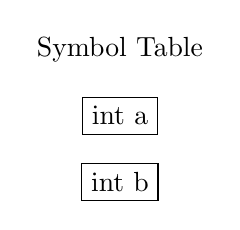
\begin{tikzpicture}
  \node at (-10pc, -8pc) {Symbol Table};
  \node [draw] at (-10pc,-10pc) (a) {int a};
  \node [draw] at (-10pc,-12pc) (b) {int b};
  \theast
\end{tikzpicture}

\end{frame}

%%%%%%%%%%%%%%%%%%%%%%%%%%%%%%

\begin{frame}[fragile=singleslide]
  \frametitle{Translation into 3-Address Code}

\begin{assembly}
L0: sne   $1,  a, b
    seq   $0, $1, 0
    btrue $0, L1    # while (a != b)
    sl    $3,  b, a
    seq   $2, $3, 0
    btrue $2, L4    # if (a < b)
    sub   a,   a, b # a -= b
    jmp   L5
L4: sub   b,   b, a # b -= a
L5: jmp   L0
L1: ret    a
\end{assembly}

\usebox{\gcdbox}\hfill\parbox{14pc}{\raggedright
Idealized assembly language w/ infinite registers
}

% Generated from SUIF/MachSUIF:
%
% c2s gcd.c
% do_lower gcd.suif gcd.lsuif
% do_s2m gcd.lsuif gcd.suifvm
% do_print gcd.suifvm
%
% Heavily massaged to make it readable

\end{frame}

%%%%%%%%%%%%%%%%%%%%%%%%%%%%%%

\begin{frame}[fragile=singleslide]
  \frametitle{Generation of 80386 Assembly}

\hfill \includegraphics[width=5pc]{80386.jpg}

\begin{assembly}
gcd:  pushl %ebp          # Save BP
      movl  %esp,%ebp
      movl  8(%ebp),%eax  # Load a from stack
      movl  12(%ebp),%edx # Load b from stack
.L8:  cmpl  %edx,%eax
      je    .L3           # while (a != b)
      jle   .L5           # if (a < b)
      subl  %edx,%eax     # a -= b
      jmp   .L8
.L5:  subl  %eax,%edx     # b -= a
      jmp   .L8
.L3:  leave               # Restore SP, BP
      ret
\end{assembly}

\end{frame}

\section{Scanning}

\subsection{Languages and Regular Expressions}

\begin{frame}
  \frametitle{Describing Tokens}

\textbf{Alphabet}: A finite set of symbols

Examples: $\{$ 0, 1 $\}$, $\{$ A, B, C, \ldots, Z $\}$, ASCII, Unicode

\vfil

\textbf{String}: A finite sequence of symbols from an alphabet

Examples: $\epsilon$ (the empty string), Stephen, $\alpha\beta\gamma$

\vfil

\textbf{Language}: A set of strings over an alphabet

Examples: $\emptyset$ (the empty language), $\{$ 1, 11, 111, 1111
$\}$, all English words, strings that start with a letter followed by
any sequence of letters and digits

\end{frame}

\begin{frame}
  \frametitle{Operations on Languages}

Let $L = \{$ $\epsilon$, wo $\}$, $M = \{$ man, men $\}$

\vfil

\textbf{Concatenation}: Strings from one followed by the other

$LM = \{$ man, men, woman, women $\}$

\vfil

\textbf{Union}: All strings from each language

$L \cup M = \{ \epsilon, $ wo, man, men $\}$

\vfil

\textbf{Kleene Closure}: Zero or more concatenations

$M^* = \{ \epsilon \} \cup M \cup MM \cup MMM \cdots = \break
 \{ \epsilon, $ man, men, manman, manmen, menman, menmen,
manmanman, manmanmen, manmenman, \ldots $\}$

\end{frame}

\begin{frame}
  \frametitle{Regular Expressions over an Alphabet $\Sigma$}

A standard way to express languages for tokens.

\begin{enumerate}

\item $\epsilon$ is a regular expression that denotes $\{\epsilon\}$

\item If $a \in \Sigma$, $a$ is an RE that denotes $\{a\}$

\item If $r$ and $s$ denote languages $L(r)$ and $L(s)$,

\begin{itemize}

\item  $(r)|(s)$ denotes $L(r) \cup L(s)$
\item $(r)(s)$ denotes $\{ tu : t \in L(r), u \in L(s) \}$
\item $(r)^*$ denotes $\cup_{i=0}^{\infty} L^i$ ($L^0 =
  \{\epsilon\}$ and $L^i = L L^{i-1}$)
\end{itemize}

\end{enumerate}

\end{frame}

\subsection{NFAs}

\begin{frame}[fragile=singleslide]
  \frametitle{Nondeterministic Finite Automata}

\begin{columns}
\begin{column}{0.4\textwidth}

``All strings containing an even number of 0's and 1's''

\vspace{2pc}

\begin{tikzpicture}
  \matrix [matrix of math nodes,
    nodes={circle,draw},
    column sep=2.5pc,
    row sep=2.5pc] {
    |[double] (A)| A & |(B)| B \\
    |(C)| C & |(D)| D \\
  };
  \begin{scope}[->, bend angle=15,bend left,inner sep=2pt]
    \draw (A) to node [above] {0} (B); 
    \draw (B) to node [below] {0} (A);
    \draw (B) to node [right] {1} (D); 
    \draw (D) to node [left]  {1} (B);
    \draw (D) to node [below] {0} (C); 
    \draw (C) to node [above] {0} (D);
    \draw (C) to node [left] {1} (A); 
    \draw (A) to node [right] {1} (C);
    \draw (A) ++ (-1.3pc,1pc) -- (A);
  \end{scope}
\end{tikzpicture}

\end{column}
\begin{column}{0.6\textwidth}

\begin{enumerate}\itemsep=0pt

\item Set of states $S:
\left\{
\begin{tikzpicture}[baseline=-4pt]
  \matrix [column sep=5pt,matrix of math nodes,nodes={circle,draw}] {
    |[double]| A & B & C & D \\ };
\end{tikzpicture}
\right\}$

\item Set of input symbols $\Sigma: \{ 0, 1 \}$

\item Transition function $\sigma : S \times \Sigma_{\epsilon} \rightarrow 2^S$

$\begin{array}{c|ccc}
\textbf{state} & \epsilon & 0 & 1 \\
\hline
A & \emptyset & \{B\} & \{C\} \\
B & \emptyset & \{A\} & \{D\} \\
C & \emptyset & \{D\} & \{A\} \\
D & \emptyset & \{C\} & \{B\} \\
\end{array}
$

\item Start state $s_0 :

\begin{tikzpicture}[baseline=-4pt]
  \node [draw,circle,double] {$A$};
\end{tikzpicture}
 $

\item Set of accepting states $F:
\left\{

\begin{tikzpicture}[baseline=-4pt]
  \node [draw,circle,double] {$A$};
\end{tikzpicture}
\right\}$

\end{enumerate}

\end{column}
\end{columns}

\end{frame}

\begin{frame}[fragile=singleslide]
  \frametitle{The Language induced by an NFA}

An NFA accepts an input string $x$ iff there is a path from the start
state to an accepting state that ``spells out'' $x$.

\vspace{2pc}

\begin{center}
\begin{tikzpicture}
  \matrix [matrix of math nodes,
    nodes={circle,draw},
    column sep=2.5pc,
    row sep=2.5pc] {
    |[double] (A)| A & |(B)| B \\
    |(C)| C & |(D)| D \\
  };
  \begin{scope}[->, bend angle=15,bend left,inner sep=2pt]
    \draw (A) to node [above] {0} (B); 
    \draw (B) to node [below] {0} (A);
    \draw (B) to node [right] {1} (D); 
    \draw (D) to node [left]  {1} (B);
    \draw (D) to node [below] {0} (C); 
    \draw (C) to node [above] {0} (D);
    \draw (C) to node [left] {1} (A); 
    \draw (A) to node [right] {1} (C);
    \draw (A) ++ (-1.3pc,1pc) -- (A);
  \end{scope}
\end{tikzpicture}
\end{center}

Show that the string ``010010'' is accepted.

\begin{tikzpicture}
  \matrix (z) [matrix of math nodes,
    nodes={circle,draw},
    column sep=1.5pc] {
    |[double]| A & B & D & C & D & B & |[double]| A \\
  };
  \begin{scope}[->,every node/.style={above}]
    \draw (z-1-1) -- node {0} (z-1-2);
    \draw (z-1-2) -- node {1} (z-1-3);
    \draw (z-1-3) -- node {0} (z-1-4);
    \draw (z-1-4) -- node {0} (z-1-5);
    \draw (z-1-5) -- node {1} (z-1-6);
    \draw (z-1-6) -- node {0} (z-1-7);
  \end{scope}
\end{tikzpicture}

\end{frame}

\subsection{Translating REs into NFAs}

\begin{frame}[fragile=singleslide]
  \frametitle{Translating REs into NFAs}

\tikzset{every matrix/.style={matrix of math nodes,
                              nodes={circle,minimum size=1pc,draw}},
         initial text={},
         every state/.style={minimum size=1.5pc,fill=white},
         group/.style={ellipse,draw,fill=black!10,minimum height=2.7pc, inner sep=-5pt},
         node distance=0.5pc and 2pc}

\begin{tabular}{ccc}
$a$ &
\begin{tikzpicture}[baseline=-4pt]
  \node[state,initial]              (A) {};
  \node[state,accepting,right=of A] (B) {};
  \path [->] (A) edge node [above] {$a$} (B);
\end{tikzpicture}
&
Symbol
\\[1pc]
$r_1 r_2$ &
\begin{tikzpicture}[baseline=-4pt]
  \node [state,initial]              (A) {};
  \node [state,right=of A]           (B) {};
  \node [state,accepting,right=of B] (C) {};
  \begin{pgfonlayer}{background}
    \node [group,fit=(A) (B)] {$r_1$};
    \node [group,fit=(B) (C)] {$r_2$};
  \end{pgfonlayer}
  \node [group,fill=none,fit=(A) (B)] {$r_1$};
\end{tikzpicture}
&
Sequence
\\[2pc]
$r_1 | r_2$ &
\begin{tikzpicture}[baseline=-4pt]
  \node [state,initial]              (A) {};
  \node [state,above right=of A]     (B) {};
  \node [state,right=of B]           (C) {};
  \node [state,accepting,below right=of C] (D) {};
  \node [state,below right=of A]     (E) {};
  \node [state,right=of E]     (F) {};
  \begin{pgfonlayer}{background}
    \node [group,fit=(B) (C)] {$r_1$};
    \node [group,fit=(E) (F)] {$r_2$};
  \end{pgfonlayer}
  \path [->] (A) edge node [above left] {$\epsilon$} (B)
             (A) edge node [below left] {$\epsilon$} (E)
             (C) edge node [above right] {$\epsilon$} (D)
             (F) edge node [below right] {$\epsilon$} (D);
\end{tikzpicture}
&
Choice
\\[3pc]
$(r)^*$ &
\begin{tikzpicture}[baseline=-4pt]
  \node [state,initial]              (A) {};
  \node [state,right=of A]           (B) {};
  \node [state,right=of B]           (C) {};
  \node [state,accepting,right=of C] (D) {};
  \begin{pgfonlayer}{background}
    \node [group,fit=(B) (C)] {$r$};
  \end{pgfonlayer}
  \path [->] (A) edge              node [above] {$\epsilon$} (B)
             (C) edge              node [above] {$\epsilon$} (D)
             (C) edge [bend right=80] node [above] {$\epsilon$} (B)
             (A) edge [bend right=40] node [below] {$\epsilon$} (D);
\end{tikzpicture}
&
Kleene Closure
 \\
\end{tabular}

\end{frame}

\def\filled#1{\ifx#11red\else white\fi}

\def\aabb#1#2#3#4#5#6#7#8#9{
  \begin{tikzpicture}[node distance=0.7pc and 1pc,                      
                      every state/.style={inner sep=1pt,
                        fill=white,
                        minimum size=14pt},
                        initial text={}]
    \node [state,fill=\filled#1,initial] (0) {0};
    \node [state,fill=\filled#2,right=of 0] (1) {1};
    \node [state,fill=\filled#3,above right=of 1] (2) {2};
    \node [state,fill=\filled#4,right=of 2] (3) {3};
    \node [state,fill=\filled#5,below right=of 1] (4) {4};
    \node [state,fill=\filled#6,right=of 4] (5) {5};
    \node [state,fill=\filled#7,below right=of 3] (6) {6};
    \node [state,fill=\filled#8,right=of 6] (7) {7};
    \node [state,fill=\filled#9,right=of 7] (8) {8};
\aabbtwo
}

\def\aabbtwo#1#2{
    \node [state,fill=\filled#1,right=of 8] (9) {9};
    \node [state,fill=\filled#2,accepting,right=of 9] (10) {10};
    \path [->] (0) edge node [above] {$\epsilon$} (1)
               (1) edge node [above left] {$\epsilon$} (2)
               (2) edge node [above] {$a$} (3)
               (1) edge node [below left] {$\epsilon$} (4)
               (4) edge node [below] {$b$} (5)            
               (3) edge node [above right] {$\epsilon$} (6)
               (5) edge node [below right] {$\epsilon$} (6)
               (6) edge node [above] {$\epsilon$} (7)
               (7) edge node [above] {$a$} (8)
               (8) edge node [above] {$b$} (9)
               (9) edge node [above] {$b$} (10)
               (6) edge [bend right=90,looseness=1.5] node [above] {$\epsilon$} (1)
               (0) edge [bend right=70] node [below] {$\epsilon$} (7)
            ;
  \end{tikzpicture}
}

\begin{frame}[fragile=singleslide]
  \frametitle{Translating REs into NFAs}

Example: Translate $(a|b)^*abb$ into an NFA. Answer:

\aabb00000000000

Show that the string ``$aabb$'' is accepted. Answer:

\begin{tikzpicture}[node distance=1pc,every state/.style={inner sep=1pt,minimum size=14pt},
    initial text={}]
  \node [state,initial] (0) {0};
  \node [state,right=of 0] (1) {1};
  \node [state,right=of 1] (2) {2};
  \node [state,right=of 2] (3) {3};
  \node [state,right=of 3] (6) {6};
  \node [state,right=of 6] (7) {7};
  \node [state,right=of 7] (8) {8};
  \node [state,right=of 8] (9) {9};
  \node [state,right=of 9,accepting] (10) {10};
  \path [->] (0) edge node [above] {$\epsilon$} (1)
             (1) edge node [above] {$\epsilon$} (2)
             (2) edge node [above] {$a$} (3)
             (3) edge node [above] {$\epsilon$} (6)
             (6) edge node [above] {$\epsilon$} (7)
             (7) edge node [above] {$a$} (8)
             (8) edge node [above] {$b$} (9)
             (9) edge node [above] {$b$} (10)
  ;
\end{tikzpicture}

\end{frame}

\begin{frame}
  \frametitle{Simulating NFAs}

Problem: you must follow the ``right'' arcs to show that a string is
accepted.  How do you know which arc is right?

Solution: follow them all and sort it out later.

``Two-stack'' NFA simulation algorithm:

\begin{enumerate}
\item Initial states: the $\epsilon$-closure of the start state
\item For each character $c$,
\begin{itemize}
\item New states: follow all transitions labeled $c$
\item Form the $\epsilon$-closure of the current states
\end{itemize}
\item Accept if any final state is accepting
\end{enumerate}

\end{frame}

\def\step#1#2#3{
\begin{frame}
  \frametitle{Simulating an NFA: #3}
\aabb #1
\aabb #2
\end{frame}
}
\def\point{\mathord{\cdot}}
%     01234 567890
\step{10000 000000}{11101 001000}{$\point aabb$, Start}
\step{00010 000100}{01111 011100}{$a\point abb$}
\step{00010 000100}{01111 011100}{$aa\point bb$}
\step{00000 100010}{01101 111010}{$aab\point b$}
\step{00000 100001}{01101 111001}{$aabb\point$, Done}

\begin{frame}
  \frametitle{Deterministic Finite Automata}

Restricted form of NFAs:

\begin{itemize}
\item No state has a transition on $\epsilon$
\item For each state $s$ and symbol $a$, there is at most one edge
  labeled $a$ leaving $s$.
\end{itemize}

Differs subtly from the definition used in COMS W3261 (Sipser,
\emph{Introduction to the Theory of Computation})

Very easy to check acceptance: simulate by maintaining current state.
Accept if you end up on an accepting state. Reject if you end on a
non-accepting state or if there is no transition from the current
state for the next symbol.

\end{frame}

\begin{frame}[fragile=singleslide]
  \frametitle{Deterministic Finite Automata}

\begin{ocamllex}
{
   type token = ELSE | ELSEIF
}

rule token =
  parse "else"   { ELSE }
      | "elseif" { ELSEIF }
\end{ocamllex}

\begin{tikzpicture}[node distance=1.5pc,
    every state/.style={inner sep=1pt,minimum size=14pt},
    initial text={}]
  \node [state,initial] (0) {};
  \node [state,right=of 0] (1) {};
  \node [state,right=of 1] (2) {};
  \node [state,right=of 2] (3) {};
  \node [state,right=of 3,accepting] (4) {};
  \node [state,right=of 4] (5) {};
  \node [state,right=of 5,accepting] (6) {};
  \path [->] (0) edge node [above] {e} (1)
             (1) edge node [above] {l} (2)
             (2) edge node [above] {s} (3)
             (3) edge node [above] {e} (4)
             (4) edge node [above] {i} (5)
             (5) edge node [above] {f} (6);
\end{tikzpicture}

\end{frame}


\begin{frame}[fragile=singleslide]
  \frametitle{Deterministic Finite Automata}

\begin{ocamllex}
{ type token = IF | ID of string | NUM of string }

rule token =
  parse "if"                                { IF }
      | ['a'-'z'] ['a'-'z' '0'-'9']* as lit { ID(lit) }
      | ['0'-'9']+                   as num { NUM(num) }
\end{ocamllex}

\begin{tikzpicture}
[node distance=3pc and 5pc,
    every state/.style={inner sep=1pt,minimum size=30pt},
    initial text={}]
  \node [state,initial] (start) {};
  \node [state,below right=of start,accepting] (num) {NUM};
  \node [state,above right=of start,accepting] (id1) {ID};
  \node [state,right=of id1,accepting] (if) {IF};
  \node [state,below=of if,accepting] (id2) {ID};
  \path [->] (start) edge node [below left] {0--9} (num)
             (start) edge node [above] {i} (id1)
             (start) edge node [above] {a--hj--z} (id2)
             (id1) edge node [above] {f} (if)
             (if) edge node [right] {a--z0--9} (id2)
             (id1) edge node [above,sloped] {a--eg--z0--9} (id2)
             (num) edge [loop right] node [right] {0--9} ()
             (id2) edge [loop right] node [right] {a--z0--9} ();
\end{tikzpicture}

\end{frame}

\subsection{Building a DFA from an NFA: Subset Construction}

\begin{frame}
  \frametitle{Building a DFA from an NFA}

Subset construction algorithm

Simulate the NFA for all possible inputs and track the states that
appear.

Each unique state during simulation becomes a state in the DFA.

\end{frame}

\def\aabb#1#2#3#4#5#6#7#8#9{
\begin{scope}[node distance=3pt and 2pt,
                      every state/.style={inner sep=1pt,
                        fill=white,
                        minimum size=5pt}]
    \node [state,fill=\filled#2] at ($(#1)+(left:1)$) (0) {};
    \node [state,fill=\filled#3,right=of 0] (1) {};
    \node [state,fill=\filled#4,above right=of 1] (2) {};
    \node [state,fill=\filled#5,right=of 2] (3) {};
    \node [state,fill=\filled#6,below right=of 1] (4) {};
    \node [state,fill=\filled#7,right=of 4] (5) {};
    \node [state,fill=\filled#8,below right=of 3] (6) {};
    \node [state,fill=\filled#9,right=of 6] (7) {};
\aabbtwo
}

\def\aabbtwo#1#2#3{
    \node [state,fill=\filled#1,right=of 7] (8) {};
    \node [state,fill=\filled#2,right=of 8] (9) {};
    \node [state,fill=\filled#3,accepting,right=of 9] (10) {};
    \path (0) edge node [above] {} (1)
          (1) edge node [above left] {} (2)
          (2) edge node [above] {} (3)
          (1) edge node [below left] {} (4)
          (4) edge node [below] {} (5)            
          (3) edge node [above right] {} (6)
          (5) edge node [below right] {} (6)
          (6) edge node [above] {} (7)
          (7) edge node [above] {} (8)
          (8) edge node [above] {} (9)
          (9) edge node [above] {} (10)
          (6) edge [bend right=90,looseness=2.5] node [above] {} (1)
          (0) edge [bend right=80,looseness=1.5] node [below] {} (7)
            ;
\end{scope}
}

%                  01234567890
\def\sa#1{\aabb{#1}11101001000}
\def\sb#1{\aabb{#1}01111011100}
\def\sc#1{\aabb{#1}01101111000}
\def\sd#1{\aabb{#1}01101111010}
\def\se#1{\aabb{#1}01101111001}

% sa -a-> sb -a-> sb -b-> sd -b-> se
% sa -b-> sc -b-> sc -a-> sb
% sd -a-> sb
% se -a-> sb
% se -b-> sc

\begin{frame}[t]
  \frametitle{Subset construction for $(a|b)^*abb$}
  \begin{tikzpicture}[nfastate/.style={state,inner sep=25pt},
    initial text={}]
    \node [initial,nfastate] (a) {};
    \sa{a}
    \pause
    \node [nfastate,right=of a] (b) {}; % \sb \\ };
    \sb{b}
    \node [nfastate,below=of a] (c) {}; % \sc \\ };
    \sc{c}
    \path [->] (a) edge node [above] {a} (b)
               (a) edge node [left] {b} (c);
    \pause
    \node [nfastate,right=of b] (d) {};% \sd \\ };
    \sd{d}
    \path [->,every loop/.style={looseness=3}]
               (b) edge [loop above] node [above] {a} ()
               (b) edge [bend left=20] node [above] {b} (d)
               (c) edge [loop left] node [left] {b} ()
               (c) edge node [below right] {a} (b);
    \pause
    \node [nfastate,accepting,below=of d] (e) {};% \se \\ };
    \se{e}
    \path [->]
          (d) edge [bend left=20] node[below] {a} (b)
          (d) edge node [right] {b} (e);
    \pause
    \path [->]
          (e) edge node [below left] {a} (b)
          (e) edge node [below] {b} (c);
  \end{tikzpicture}
\end{frame}

\begin{frame}
  \frametitle{Result of subset construction for $(a|b)^*abb$}
\begin{center}
  \begin{tikzpicture}[node distance=4pc,initial text={}]
    \node [initial,state] (a) {};
    \node [state,right=of a] (b) {};
    \node [state,below=of a] (c) {};
    \path [->] (a) edge node [above] {a} (b)
               (a) edge node [left] {b} (c);
    \node [state,right=of b] (d) {};
    \path [->,every loop/.style={looseness=3}]
               (b) edge [loop above] node [above] {a} ()
               (b) edge [bend left=20] node [above] {b} (d)
               (c) edge [loop left] node [left] {b} ()
               (c) edge node [below right] {a} (b);
    \node [state,accepting,below=of d] (e) {};
    \path [->]
          (d) edge [bend left=20] node[below] {a} (b)
          (d) edge node [right] {b} (e);
    \path [->]
          (e) edge node [below left] {a} (b)
          (e) edge node [below] {b} (c);
  \end{tikzpicture}

\end{center}
\end{frame}

\section{Parsing}

\subsection{Resolving Ambiguity}

\begin{frame}
  \frametitle{Ambiguous Arithmetic}

Ambiguity can be a problem in expressions.  Consider parsing

\begin{center}
\texttt{3 - 4 * 2 + 5}
\end{center}

with the grammar

\[e \rightarrow  e + e | e - e | e * e | e \mathop{/} e | N\]

\ttfamily

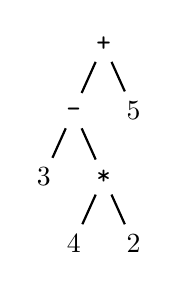
\begin{tikzpicture}[parsetree]
  \path
    \plus{\minus{\lit3}
                {\mult{\lit4}{\lit2}}}
         {\lit5}
    ;
\end{tikzpicture}
\hfil
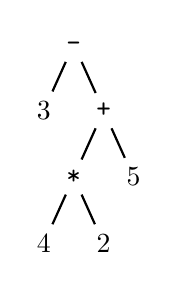
\begin{tikzpicture}[parsetree]
  \path
    \minus{\lit3}
          {\plus{\mult{\lit4}{\lit2}}
                {\lit5}}
    ;
\end{tikzpicture}
\hfil
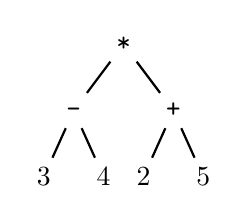
\begin{tikzpicture}[parsetree,
                 level 1/.style={sibling distance=3pc},
                 level 2/.style={sibling distance=1.8pc}]
  \path \mult{\minus{\lit3}{\lit4}}
              {\plus{\lit2}{\lit5}}
    ;
\end{tikzpicture}
\hfil
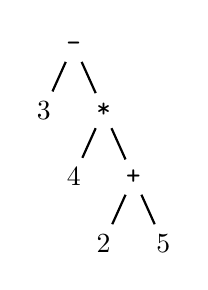
\begin{tikzpicture}[parsetree]
  \path \minus{\lit3}
              {\mult{\lit4}
                     {\plus{\lit2}{\lit5}}};
\end{tikzpicture}
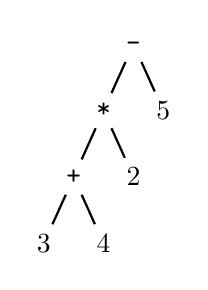
\begin{tikzpicture}[parsetree]
  \path \minus{\mult{\plus{\lit3}{\lit4}}{\lit2}}{\lit5};
\end{tikzpicture}

\end{frame}

\begin{frame}
  \frametitle{Operator Precedence}

Defines how ``sticky'' an operator is.

\begin{center}\ttfamily
1 * 2 + 3 * 4
\end{center}

\begin{minipage}{0.65\textwidth}
\texttt{*} at higher precedence than \texttt{+}:

\medskip

\texttt{(1 * 2) + (3 * 4)}
\end{minipage}
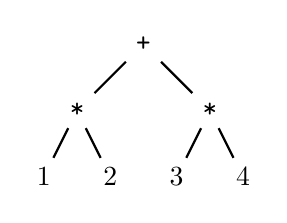
\begin{tikzpicture}[parsetree,
    level 1/.style={sibling distance=4pc},
    level 2/.style={sibling distance=2pc}]
  \path
  \plus{\mult{\lit1}{\lit2}}
       {\mult{\lit3}{\lit4}};
\end{tikzpicture}

\begin{minipage}{0.65\textwidth}
\texttt{+} at higher precedence than \texttt{*}:

\medskip

\texttt{1 * (2 + 3) * 4}
\end{minipage}
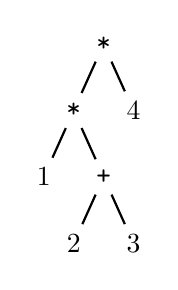
\begin{tikzpicture}[parsetree]
  \path
  \mult{\mult{\lit1}
               {\plus{\lit2}{\lit3}}}
        {\lit4};
\end{tikzpicture}
\end{frame}

\begin{frame}
  \frametitle{Associativity}

Whether to evaluate left-to-right or right-to-left

Most operators are left-associative

\begin{center}
\texttt{1 - 2 - 3 - 4}

\vspace{2pc}

\begin{tabular}{c@{\hspace{5pc}}c}
  \ttfamily
  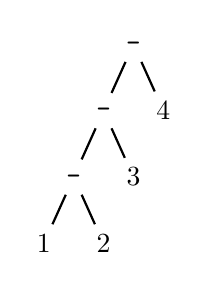
\begin{tikzpicture}[parsetree]
    \path \minus{\minus{\minus{\lit1}{\lit2}}{\lit3}}{\lit4};
  \end{tikzpicture}
&
  \ttfamily
  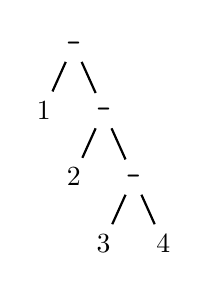
\begin{tikzpicture}[parsetree]
    \path \minus{\lit1}{\minus{\lit2}{\minus{\lit3}{\lit4}}};
  \end{tikzpicture}
\\
\\
$((1 - 2) - 3) - 4$ & $1 - (2 - (3 - 4))$ \\
\\
left associative & right associative
\end{tabular}

\end{center}

\end{frame}

\begin{frame}[fragile=singleslide]
  \frametitle{Fixing Ambiguous Grammars}

A grammar specification:

\begin{ocamlyacc}
expr :
    expr PLUS expr  
  | expr MINUS expr 
  | expr TIMES expr 
  | expr DIVIDE expr
  | NUMBER          
\end{ocamlyacc}

Ambiguous: no precedence or associativity.

Ocamlyacc's complaint: ``16 shift/reduce conflicts.''

\end{frame}

\begin{frame}[fragile=singleslide]
  \frametitle{Assigning Precedence Levels}

Split into multiple rules, one per level

\begin{ocamlyacc}
expr : expr PLUS expr  
     | expr MINUS expr 
     | term            

term : term TIMES term 
     | term DIVIDE term
     | atom            

atom  : NUMBER         
\end{ocamlyacc}

Still ambiguous: associativity not defined

Ocamlyacc's complaint: ``8 shift/reduce conflicts.''

\end{frame}

\begin{frame}[fragile=singleslide]
  \frametitle{Assigning Associativity}

Make one side the next level of precedence

\begin{ocamlyacc}
expr : expr PLUS term  
     | expr MINUS term 
     | term            

term : term TIMES atom 
     | term DIVIDE atom
     | atom            

atom  : NUMBER         
\end{ocamlyacc}

This is left-associative.

No shift/reduce conflicts.

\end{frame}

\renewcommand{\id}{\textbf{Id}}

\newcommand{\handle}[3]{
  \begin{tikzpicture}
    \node [inner sep=1pt] (n1) {$#1$};
    \node [inner sep=1pt,anchor=base west] (n2) at (n1.base east) {$#2$};
    \node [inner sep=1pt,anchor=base west] (n1) at (n2.base east) {$#3$};
    \begin{pgfonlayer}{background}
      \draw [red!70,line width=2pt,rounded corners]
      ($(n2.north east) + (1pt,1pt)$) --
      ($(n2.north west) + (-1pt,1pt)$) --
      ($(n2.south west) + (-1pt,-1pt)$) --
      ($(n2.south east) + (1pt,-1pt)$) -- cycle
      ;
    \end{pgfonlayer}
  \end{tikzpicture}
}

\newcommand{\expand}[3]{
    \fill [even odd rule,red,path fading=fade up]
    (#1.north west)  [rounded corners] -- (#1.south west) --
    (#2.north west) -- (#2.south west) -- (#3.south east) --
    (#3.north east) -- (#1.south east) -- (#1.north east)
    -- cycle
    ($(#3.north east) + (-1pt,-1pt)$) --
    ($(#2.north west) + (1pt,-1pt)$) --
    ($(#2.south west) + (1pt,1pt)$) --
    ($(#3.south east) + (-1pt,1pt)$) -- cycle
    ;
}

\newcommand{\expandup}[3]{
    \fill [even odd rule,red,path fading=fade down]
    (#1.south west)  [rounded corners] -- (#1.north west) --
    (#2.south west) -- (#2.north west) -- (#3.north east) --
    (#3.south east) -- (#1.north east) -- (#1.south east)
    -- cycle
    ($(#3.south east) + (-1pt,1pt)$) --
    ($(#2.south west) + (1pt,1pt)$) --
    ($(#2.north west) + (1pt,-1pt)$) --
    ($(#3.north east) + (-1pt,-1pt)$) -- cycle
    ;
}

\newcommand{\grammarone}{
\renewcommand{\arraystretch}{1}
$\begin{array}[t]{@{}l@{\,}r@{\,}c@{\,}l@{}}
1: & e & \rightarrow & t + e \\
2: & e & \rightarrow & t \\
3: & t & \rightarrow & \id\ * t \\
4: & t & \rightarrow & \id
\end{array}$
}


\newenvironment{parsermoves}{
\begingroup
\small
\renewcommand{\arraystretch}{0.8}
\newcommand{\s}[2]{%
  \begin{pspicture}(10pt,10pt)
    \psframe(0,-5pt)(8pt,5pt)
    \rput(4pt,2pt){\tiny##1}
    \rput(4pt,-2pt){\tiny##2}
  \end{pspicture}}
\begin{tabular}[t]{l@{}rl}
\multicolumn{1}{c}{\hbox to 5em{\hss stack\hss}} & \multicolumn{1}{c}{input}
& \multicolumn{1}{c}{action} \\
}{
\end{tabular}
\endgroup
}


\newsavebox{\rightmostDerivation}
\begin{lrbox}{\rightmostDerivation}
  \begin{tikzpicture}[every node/.style={anchor=base,inner sep=2pt},
                      node distance=0pt]
  \node (t1) {$e$};
  \node [below=of t1,matrix of math nodes,inner sep=0pt] (t2) {
    t & + & |(t3)| e \\ };
  \node [below=of t2,matrix of math nodes] (t4) {
    t & + & |(t5)| t \\ };
  \node [below=of t4,matrix of math nodes] (t6) {
    |(t8)| t & + & |(t7)| \id \\ };
  \node [below=of t6,matrix of math nodes] (t9) {
    |(t10)| \id & * & |(t10a)| t & + & \id \\ };
  \node [below=of t9,matrix of math nodes] (t11) {
    \id & * & |(t12)| \id & + & \id \\ };
  \begin{pgfonlayer}{background}
    \expand{t1}{t2}{t2}
    \expand{t3}{t5}{t5}
    \expand{t5}{t7}{t7}
    \expand{t8}{t10}{t10a}
    \expand{t10a}{t12}{t12}
  \end{pgfonlayer}
      \end{tikzpicture}
\end{lrbox}

\newsavebox{\automataPatterns}
\begin{lrbox}{\automataPatterns}
\footnotesize\renewcommand{\arraystretch}{0.1}
\begin{tabular}[t]{l}
\handle{\id * \id * \cdots * }{\id * t}{\cdots} \\
\handle{\id * \id * \cdots * }{\id}{\cdots} \\
\handle{t + t + \cdots + }{t+e}{} \\
\handle{t + t + \cdots + t + }{\id}{} \\
\handle{t + t + \cdots + t + \id * \id * \cdots * }{\id * t}{} \\
\handle{t + t + \cdots + }{t}{} \\
\end{tabular}
\end{lrbox}

\subsection{Rightmost and Reverse-Rightmost Derivations}

\begin{frame}[t,fragile]
  \frametitle{Rightmost Derivation of $\id * \id + \id$}

\begin{columns}
  \begin{column}{0.3\textwidth}
    \grammarone
  \end{column}
  \begin{column}{0.7\textwidth}

\begin{center}
\begin{tikzpicture}[every node/.style={anchor=base,inner sep=2pt},
  node distance=0.3pc]
  \node (t1) {$e$};
  \node [below=of t1,matrix of math nodes,inner sep=0pt] (t2) {
    t & + & |(t3)| e \\ };
  \node [below=of t2,matrix of math nodes] (t4) {
    t & + & |(t5)| t \\ };
  \node [below=of t4,matrix of math nodes] (t6) {
    |(t8)| t & + & |(t7)| \id \\ };
  \node [below=of t6,matrix of math nodes] (t9) {
    |(t10)| \id & * & |(t10a)| t & + & \id \\ };
  \node [below=of t9,matrix of math nodes] (t11) {
    \id & * & |(t12)| \id & + & \id \\ };
  \begin{pgfonlayer}{background}
    \expand{t1}{t2}{t2}
    \expand{t3}{t5}{t5}
    \expand{t5}{t7}{t7}
    \expand{t8}{t10}{t10a}
    \expand{t10a}{t12}{t12}
  \end{pgfonlayer}
\end{tikzpicture}
\end{center}
  \end{column}
\end{columns}

\begin{center}

At each step, expand the \emph{rightmost} nonterminal.

\vspace{1pc}

\begin{tikzpicture}[node distance=0.5pc]
  \node (nt) {nonterminal};
  \node [below=of nt] (h)
        {``handle'': The right side of a production};
  \begin{pgfonlayer}{background}
    \expand{nt}{h}{h}
  \end{pgfonlayer}
\end{tikzpicture}

Fun and interesting fact: there is exactly one rightmost expansion if
the grammar is unambigious.

\end{center}

\end{frame}

\begin{frame}[t,fragile]
  \frametitle{Rightmost Derivation: What to Expand}

\begin{columns}
  \begin{column}{0.3\textwidth}
    \grammarone
  \end{column}
  \begin{column}{0.7\textwidth}
    \begin{center}
      \usebox{\rightmostDerivation}
    \end{center}
  \end{column}
\end{columns}

\begin{center}
  \begin{tikzpicture}[every node/.style={inner sep=2pt}]
  \node [anchor=east] (t1) {$e$};
  \node [anchor=east,matrix of math nodes,inner sep=0pt] at (0,-1.5pc) (t2) {
    t & + & |(t3)| e \\ };
  \node [anchor=east,matrix of math nodes] at (0,-3pc) (t4) {
    t & + & |(t5)| t \\ };
  \node [anchor=t8.east,matrix of math nodes] at (0,-4.5pc) (t6) {
    |(t8)| t & + & |(t7)| \id \\ };
  \node [anchor=t10a.east,matrix of math nodes] at (0,-6pc) (t9) {
    |(t10)| \id & * & |(t10a)| t & + & \id \\ };
  \node [anchor=west,matrix of math nodes] at (0,-7.5pc) (t11) {
    \id & * & |(t12)| \id & + & \id \\ };
  \begin{pgfonlayer}{background}
    \fill [black!10] (t1.north east) [rounded corners] rectangle +(-6pc,-9pc)
          node [black,below right] {Expand here $\uparrow$};
    \fill [black!10] ($(t1.north east) + (2pt,0)$)
          [rounded corners] rectangle +(6pc,-9pc)
          node [black,below left] {Terminals only};
    \expand{t1}{t2}{t2}
    \expand{t3}{t5}{t5}
    \expand{t5}{t7}{t7}
    \expand{t8}{t10}{t10a}
    \expand{t10a}{t12}{t12}
  \end{pgfonlayer}
  \end{tikzpicture}
\end{center}

\end{frame}

\begin{frame}[t,fragile]
  \frametitle{Reverse Rightmost Derivation}

\begin{columns}
  \begin{column}{0.3\textwidth}
    \grammarone
  \end{column}
  \begin{column}{0.7\textwidth}
    \begin{center}
      \usebox{\rightmostDerivation}
    \end{center}
  \end{column}
\end{columns}

\begin{center}
  \begin{tikzpicture}[every node/.style={inner sep=1pt}]
  \node [anchor=west,matrix of math nodes] at (0,0) (t11) {
    \id & * & |(t12)| \id & + & \id \\ };
  \node (h10) at (9.8pc,0pc) {\id};
  \node (h9) at (9.8pc,-1.5pc) {$t$};
  \draw (h10) to (h9);
  \node [anchor=t10a.east,matrix of math nodes] at (0,-1.5pc) (t9) {
    |(t10)| \id & * & |(t10a)| t & + & \id \\ };
  \node (h8) at (8.8pc,-1.5pc) {$*$};
  \node (h7) at (7.8pc,-1.5pc) {\id};
  \node (h6) at (8.8pc,-3pc) {$t$};
  \draw (h6) to (h7)
        (h6) to (h8)
        (h6) to (h9);
  \node [anchor=t8.east,matrix of math nodes] at (0,-3pc) (t6) {
    |(t8)| t & + & |(t7)| \id \\ };
  \node (h5) at (10.6pc,-3pc) {\id};
  \node (h4) at (10.6pc,-4.5pc) {$t$};
  \draw (h4) to (h5);
  \node [anchor=east,matrix of math nodes] at (0,-4.5pc) (t4) {
    t & + & |(t5)| t \\ };
  \node (h3) at (10.6pc,-6pc) {$e$};
  \draw (h3) to (h4);
  \node [anchor=east,matrix of math nodes] at (0,-6pc) (t2) {
    t & + & |(t3)| e \\ };
  \node (h1) at (8.8pc,-7.5pc) {$e$};
  \node (h2) at (9.6pc,-6pc) {$+$};
  \draw (h1) to (h2)
        (h1) to (h3)
        (h1) to (h6);
  \node [anchor=east] (t1) at (0,-7.5pc) {$e$};
  \begin{pgfonlayer}{background}
    \fill [black!10] (t11.north west) [rounded corners] rectangle +(-6pc,-9pc)
          node [black,below right] {viable prefixes};
    \fill [black!10] ($(t11.north west) + (2pt,0)$)
          [rounded corners] rectangle +(6pc,-9pc)
          node [black,below left] {terminals};
    \expandup{t1}{t2}{t2}
    \expandup{t3}{t5}{t5}
    \expandup{t5}{t7}{t7}
    \expandup{t8}{t10}{t10a}
    \expandup{t10a}{t12}{t12}
  \end{pgfonlayer}
  \end{tikzpicture}
\end{center}

\end{frame}

\begin{frame}[fragile=singleslide,t]
  \frametitle{Shift/Reduce Parsing Using an Oracle}

\begin{columns}
  \begin{column}{0.3\textwidth}
    \grammarone
  \end{column}
  \begin{column}{0.7\textwidth}
    \begin{center}
      \usebox{\rightmostDerivation}
    \end{center}
  \end{column}
\end{columns}

\begin{center}
  \begin{tikzpicture}[every node/.style={inner sep=1pt}]
  \node [anchor=west,matrix of math nodes] at (0,0) (t0) {
    \id & * & \id & + & \id \\ };
  \node [anchor=west] at (6.5pc,0pc) {shift};
%  \pause
  \node [anchor=t1.east,matrix of math nodes] at (0,-1pc) {
    |(t1)| \id & * & \id & + & \id \\ };
  \node [anchor=west] at (6.5pc,-1pc) {shift};
%  \pause
  \node [anchor=t2.east,matrix of math nodes] at (0,-2pc) {
    \id & |(t2)| * & \id & + & \id \\ };
  \node [anchor=west] at (6.5pc,-2pc) {shift};
%  \pause
  \node [anchor=t3.east,matrix of math nodes] at (0,-3pc) {
    \id & * &  |(t3)| \id & + & \id \\ };
  \node [anchor=west] at (6.5pc,-3pc) {reduce 4};
%  \pause
  \node [anchor=t4.east,matrix of math nodes] at (0,-4pc) {
    |(t5)| \id & * &  |(t4)| t & + & \id \\ };
  \node [anchor=west] at (6.5pc,-4pc) {reduce 3};
%  \pause
  \node [anchor=t6.east,matrix of math nodes] at (0,-5pc) {
    |(t6)| t & + & \id \\ };
  \node [anchor=west] at (6.5pc,-5pc) {shift};
%  \pause
  \node [anchor=t7.east,matrix of math nodes] at (0,-6pc) {
    t & |(t7)| + & \id \\ };
  \node [anchor=west] at (6.5pc,-6pc) {shift};
%  \pause
  \node [anchor=t8.east,matrix of math nodes] at (0,-7pc) {
    t & + & |(t8)| \id \\ };
  \node [anchor=west] at (6.5pc,-7pc) {reduce 4};
%  \pause
  \node [anchor=t9.east,matrix of math nodes] at (0,-8pc) {
    t & + & |(t9)| t \\ };
  \node [anchor=west] at (6.5pc,-8pc) {reduce 2};
%  \pause
  \node [anchor=t10.east,matrix of math nodes] at (0,-9pc) {
    |(t11)| t & + & |(t10)| e \\ };
  \node [anchor=west] at (6.5pc,-9pc) {reduce 1};
%  \pause
  \node [anchor=east] at (0,-10pc) (t12) {$e$};
  \node [anchor=west] at (6.5pc,-10pc) {accept};
  \begin{pgfonlayer}{background}
    \fill [black!10] (t0.north west) [rounded corners] rectangle +(-6pc,-11pc)
          node [black,below right] {stack};
    \fill [black!10] ($(t0.north west) + (2pt,0)$)
          [rounded corners] rectangle +(6pc,-11pc)
          node [black,below left] {input};
    \expandup{t4}{t3}{t3}
    \expandup{t6}{t5}{t4}
    \expandup{t9}{t8}{t8}
    \expandup{t10}{t9}{t9}
    \expandup{t12}{t11}{t10}
  \end{pgfonlayer}
  \end{tikzpicture}
\end{center}

\end{frame}

\begin{frame}
  \frametitle{Handle Hunting}

\textbf{Right Sentential Form:} any step in a rightmost derivation

\textbf{Handle:} in a sentential form, a RHS of a rule that, when
rewritten, yields the previous step in a rightmost derivation.

The big question in shift/reduce parsing:

\begin{center}
When is there a handle on the top of the stack?
\end{center}

Enumerate all the right-sentential forms and pattern-match against
them? \emph{Usually infinite in number, but let's try anyway.}

\end{frame}

\begin{frame}
  \frametitle{The Handle-Identifying Automaton}

Magical result, due to Knuth:  \emph{An automaton suffices to locate a handle
  in a right-sentential form.}

\begin{columns}
  \begin{column}{0.6\textwidth}
    \usebox{\automataPatterns}
  \end{column}
  \begin{column}{0.4\textwidth}
\begin{tikzpicture}[node distance=1.2pc and 2pc,initial text={},
    every state/.style={minimum size=28pt}]
  \node [state,initial] (S0) {};
  \node [state,below=of S0,accepting] (S1) {$\id$};
  \node [state,right=of S0,accepting] (S2) {$t$};
  \node [state,below=of S1] (S3) {};
  \node [state,below=of S2] (S4) {};
  \node [state,below=of S3,accepting] (S5) {$\id * t$};
  \node [state,below=of S4,accepting] (S6) {$t + e$};
  \node [state,above=of S0,accepting] (S7) {$e$};
  \path [->]
     (S0) edge node [above] {$t$} (S2)
     (S2) edge [bend left] node [right] {$+$} (S4)
     (S4) edge [bend left] node [left] {$t$} (S2)
     (S4) edge node [right] {$e$} (S6)
     (S4) edge node [above] {$\id$} (S1)
     (S0) edge node [right] {$\id$} (S1)   
     (S1) edge [bend left] node [right] {$*$} (S3)
     (S3) edge [bend left] node [left] {$\id$} (S1)
     (S3) edge node [right] {$t$} (S5)
     (S0) edge node [right] {$e$} (S7)
  ;
\end{tikzpicture}
  \end{column}
\end{columns}

\end{frame}


\subsection{Building the LR(0) Automaton}

\begin{frame}
  \frametitle{Building the Initial State of the LR(0) Automaton}

\grammarone\hfill\framebox{$\begin{array}{l}
    e' \rightarrow \pac e \\
    \onslide<2->{e \rightarrow \pac t + e \\
    e \rightarrow \pac t \\}
    \onslide<3->{t \rightarrow \pac \id * t \\
    t \rightarrow \pac \id}
  \end{array}$
}

Key idea: automata identify viable prefixes of right sentential forms.
Each state is an equivalence class of possible places in productions.

At the beginning, any viable prefix must be at the beginning of a
string expanded from $e$.  We write this condition ``$e' \rightarrow
\pac e$''

\onslide<2->{There are two choices for what an $e$ may expand to:
  $t+e$ and $t$.  So when $e' \rightarrow \pac e$, $e \rightarrow \pac
  t+e$ and $e \rightarrow \pac t$ are also true, i.e., it must start
  with a string expanded from $t$.}

\onslide<3->{Similarly, $t$ must be either $\id * t$ or $\id$, so $t
  \rightarrow \pac \id * t$ and $t \rightarrow \pac \id$.

This reasoning is a \emph{closure} operation like $\epsilon$-closure
in subset construction.
}

\end{frame}

\begin{frame}
  \frametitle{Building the LR(0) Automaton}

\begin{columns}
  \begin{column}{0.5\textwidth}
\small
\begin{tikzpicture}[node distance=1.5pc]

  \node [draw] (S0) {$\textbf{S0}: \begin{array}{@{}l@{}}
    e' \rightarrow \pac e \\
    e \rightarrow \pac t + e \\
    e \rightarrow \pac t \\
    t \rightarrow \pac \id * t \\
    t \rightarrow \pac \id
  \end{array}$};

  \onslide<2->{

    \node [draw,accepting,below=of S0] (S1) {$\textbf{S1}: \begin{array}{@{}l@{}}
        t \rightarrow \id \pac * t \\
        t \rightarrow \id \pac
      \end{array}$};

    \node [draw,accepting,above=of S0] (S7) {$\textbf{S7}:\ e'
      \rightarrow e \pac$};

    \node [draw,accepting,right=of S0] (S2) {$\textbf{S2}: \begin{array}{@{}l@{}}
        e \rightarrow t \pac + e \\
        e \rightarrow t \pac
      \end{array}$};

     \path [->]
     (S0) edge node [right] {$e$} (S7)
     (S0) edge node [right] {$\id$} (S1)
     (S0) edge node [above] {$t$} (S2)
     ;
  }

  \onslide <3->{
    \node [draw,below=of S1] (S3) {$\textbf{S3}: \begin{array}{@{}l@{}}
        t \rightarrow \id * \pac t \\
        \onslide<4->{
        t \rightarrow \pac \id * t \\
        t \rightarrow \pac \id}
      \end{array}$};

    \node [draw,right=of S2] (S4)
          {$\textbf{S4}: \begin{array}{@{}l@{}}
              e \rightarrow t + \pac e \\
              \onslide<4->{
              e \rightarrow \pac t + e \\
              e \rightarrow \pac t \\
              t \rightarrow \pac \id * t \\
              t \rightarrow \pac \id}
            \end{array}$};

    \path [->] (S1) edge [bend left=10] node [right] {$*$} (S3)
               (S2) edge [bend left=10] node [above] {$+$} (S4);
  }

  \onslide<5->{

    \node [draw,accepting,right=of S3] (S5) {$\textbf{S5}:\ t
      \rightarrow \id * t \pac$};

    \path [->]
      (S3) edge node [above] {$t$} (S5)
      (S3) edge [bend left=10] node [left] {$\id$} (S1);

    \node [draw,accepting, below=of S4] (S6)
          {$\textbf{S6}:\ e \rightarrow t + e \pac$};

    \path [->] (S4) edge [bend left=10] node [below] {$t$} (S2)
      (S4) edge [bend left=10] node [above] {$\id$} (S1)
      (S4) edge node [right] {$e$} (S6);
  }

  \onslide<2>{

    \node [above,text width=6.5pc,text ragged] at (S2.north)
          {\footnotesize\emph{``Just passed a
              prefix ending in a string derived from $t$''}};

    \node [below,text width=6.5pc,text badly ragged] at (S1.south)
          {\footnotesize\emph{``Just passed a prefix that ended in an \id''}};

    \node [above,text width=8pc,text ragged] at (S7.north)
          {\footnotesize\emph{``Just passed a string derived from $e$''}};
  }
\end{tikzpicture}
  \end{column}
  \begin{column}{0.5\textwidth}
    \onslide<1-2>{
      The first state suggests a viable prefix can start as any string
      derived from $e$, any string derived from $t$, or $\id$.
      \medskip
    }

    \onslide<2>{
      The items for these three states come from advancing the $\pac$
      across each thing, then performing the closure operation
      (vacuous here).
    }

    \onslide<3-4>{In S2, a $+$ may be next.  This gives $t + \pac e$.
      \onslide<4>{Closure adds 4 more items.}

      \medskip

      In S1, $*$ may be next, giving $\id * \pac t$
      \onslide<4>{and two others.}      
    }
  \end{column}
\end{columns}

\end{frame}

\subsection{First and Follow}

\newcommand\first{\textsc{first}}
\newcommand\follow{\textsc{follow}}

\begin{frame}{The \first{} function}

\parskip=5pt

If you can derive a string that starts with terminal $t$ from a
sequence of terminals and nonterminals $\alpha$, then $t \in
\first(\alpha)$.

\begin{enumerate}
\item If $X$ is a terminal, $\first(X) = \{ X \}$.

\item If $X \rightarrow \epsilon$, then add $\epsilon$ to $\first(X)$.

\item If $X \rightarrow Y_1 \cdots Y_k$ and
  $\epsilon \in \first(Y_1)$,
  $\epsilon \in \first(Y_2)$, \ldots, and $\epsilon \in
  \first(Y_{i-1})$ for $i=1,\ldots, k$ for some $k$, \\ \quad add
  $\first(Y_i) - \{ \epsilon \}$ to $\first(X)$

    \textcolor{red}{\emph{$X$ starts with anything that appears after
      skipping empty strings. Usually just $\first(Y_1) \in \first(X)$}}

\item If $X \rightarrow Y_1 \cdots Y_K$ and
  $\epsilon \in \first(Y_1)$,
  $\epsilon \in \first(Y_2)$, \ldots, and $\epsilon \in \first(Y_k)$, add
  $\epsilon$ to $\first(X)$

    \textcolor{red}{\emph{If all of $X$ can be empty, $X$ can be empty}}  
\end{enumerate}

\hrule

\vspace{5pt}

\begin{columns}
\begin{column}{0.3\textwidth}
\grammarone
\end{column}
\begin{column}{0.7\textwidth}
\parskip=5pt
$\first(\id) = \{ \id \}$

$\first(t) = \{ \id \}$ because $t \rightarrow \id\ * t$ and $t
  \rightarrow \id$

$\first(e) = \{ \id \}$ because $e \rightarrow t + e$, $e \rightarrow
  t$, and $\first(t) = \{ \id \}$.

\end{column}
\end{columns}

\end{frame}

\begin{frame}{First and $\epsilon$}
  $\epsilon \in \first(\alpha)$ means $\alpha$ can derive the empty
  string.

  \begin{enumerate}
\item If $X$ is a terminal, $\first(X) = \{ X \}$.

\item If $X \rightarrow \epsilon$, then add $\epsilon$ to $\first(X)$.

\item If $X \rightarrow Y_1 \cdots Y_k$ and \\
  $\epsilon \in \first(Y_1)$,
  $\epsilon \in \first(Y_2)$, \ldots, and $\epsilon \in
  \first(Y_{i-1})$ \\ for $i=1,\ldots, k$ for some $k$, \\ \quad add
  $\first(Y_i) - \{ \epsilon \}$ to $\first(X)$

\item If $X \rightarrow Y_1 \cdots Y_K$ and \\
  $\epsilon \in \first(Y_1)$,
  $\epsilon \in \first(Y_2)$, \ldots, and $\epsilon \in \first(Y_k)$, \\ \quad add
  $\epsilon$ to $\first(X)$
      \end{enumerate}

  \begin{columns}
    \begin{column}{0.15\textwidth}
      $\begin{array}{l@{\,}l@{\,}l}
        X & \rightarrow & Y Z a \\
        Y & \rightarrow & \\
        Y & \rightarrow & b \\
        Z & \rightarrow & c \\
        Z & \rightarrow & W \\
        W & \rightarrow & \\
        W & \rightarrow & d \\
      \end{array}$
    \end{column}
    \begin{column}{0.85\textwidth}
$\begin{array}{ll}

\first(b) = \{ b \}\quad \first(c) = \{ c \}\quad \first(d) = \{ d \} & (1) \\
  
\first(W) = \{ \epsilon \} \cup \first(d) = \{ \epsilon, d \} & (2, 3) \\

\first(Z) = \first(c) \cup (\first(W) - \{\epsilon\}) \cup \{ \epsilon \} = \{ \epsilon, c, d \} & (3, 3, 4) \\

\first(Y) = \{ \epsilon \} \cup \{ b \} = \{ \epsilon, b \} & (2, 3) \\

\first(X) = (\first(Y) - \{\epsilon\}) \cup (\first(Z) - \{\epsilon\}) \cup \\
 \quad \quad \quad \quad \quad \first(a) = \{a, b, c, d\} & (3, 3, 3) \\
      \end{array}$
    \end{column}
  \end{columns}
  
\end{frame}

\begin{frame}{The \textsc{follow} function}

If $t$ is a terminal, $A$ is a nonterminal, and $\cdots A t \cdots$
can be derived, then $t \in \follow(A)$.

\begin{enumerate}
\item Add \$ (``end-of-input'') to $\follow(S)$ (start symbol).

  \textcolor{red}{\emph{End-of-input comes after the start symbol}}

\item For each prod.\ $\rightarrow \cdots A \alpha$, add
  $\first(\alpha) - \{ \epsilon \}$ to $\follow(A)$.

  \textcolor{red}{\emph{$A$ is followed by the first thing after it}}

\item For each prod.\ $A \rightarrow \cdots B$ or $A \rightarrow
  \cdots B \alpha$ where $\epsilon \in \first(\alpha)$, then add
  everything in $\follow(A)$ to $\follow(B)$.

  \textcolor{red}{\emph{If $B$ appears at the end of a production, it
      can be followed by whatever follows that production}}

\end{enumerate}

\hrule

\vspace{5pt}

\begin{columns}
\begin{column}[t]{0.3\textwidth}
\grammarone

$\first(t) = \{\id\}$

$\first(e) = \{\id\}$
\end{column}
\begin{column}[t]{0.7\textwidth}
$\follow(e) = \{ \$ \}$

$\follow(t) = \{ \uncover<2->{+} \uncover<3->{, \$} \}$

\medskip

\only<1>{%
\emph{1. Because $e$ is the start symbol}
}%
\only<2>{%
\emph{2. Because $e \rightarrow \underbar{t} + e$ and $\first(+) = \{+\}$}
}%
\only<3>{%
\emph{3. Because $e \rightarrow \underline{t}$ and $\$ \in \follow(e)$}
}%
\only<4>{%
Fixed-point reached: applying any rule does not change any set
}

\end{column}
\end{columns}

\end{frame}

\def\highlight<#1>#2{
  {\temporal<#1>{\color{black!30}}{}{\color{black!30}}#2}
}

\subsection{Building an SLR Parsing Table}

\begin{frame}[t]
  \frametitle{Converting the LR(0) Automaton to an SLR Parsing Table}

\begin{columns}
  \begin{column}{0.5\textwidth}
\begin{tikzpicture}[node distance=2pc,initial text={}]
  \highlight<1>{\node [draw,initial] (S0) {\textbf{S0}};}
  \highlight<1,2,4,5>{\node [draw,below=of S0,accepting] (S1)
    {\textbf{S1}: $t \rightarrow \id\pac$};}
  \highlight<1,3,5>{\node [draw,right=of S0,accepting] (S2)
    {\textbf{S2}: $e \rightarrow t\pac$};}
  \highlight<2,4>{\node [draw,below=of S1] (S3) {\textbf{S3}};}
  \highlight<3,5>{\node [draw,below=of S2] (S4) {\textbf{S4}};}
  \highlight<4,6>{\node [draw,below=of S3,accepting] (S5)
        {\textbf{S5}: $t \rightarrow \id * t\pac$};}
  \highlight<5,7>{\node [draw,below=of S4,accepting] (S6)
        {\textbf{S6}: $e \rightarrow t + e\pac$};}
  \highlight<1,8>{\node [draw,above=of S0,accepting] (S7)
        {\textbf{S7}: $e' \rightarrow e\pac$};}
 \highlight<1>{\path [->]
  (S0) edge node [above] {$t$} (S2)
  (S0) edge node [right] {$\id$} (S1)   
  (S0) edge node [right] {$e$} (S7);}
 \highlight<2>{\path [->] (S1) edge [bend left] node [right] {$*$} (S3);}
 \highlight<3>{\path [->] (S2) edge [bend left] node [right] {$+$} (S4);}
 \highlight<4>{\path [->]
   (S3) edge [bend left] node [left] {$\id$} (S1)
   (S3) edge node [right] {$t$} (S5);}
 \highlight<5>{\path [->]
   (S4) edge [bend left] node [left] {$t$} (S2)
   (S4) edge node [right] {$e$} (S6)
   (S4) edge node [above] {$\id$} (S1);}

  \node [right=of S7] {\grammarone};
\end{tikzpicture}
  \end{column}
  \begin{column}[t]{0.5\textwidth}
    \small
    \begin{tabular}{c|cccc|cc}
      \toprule
      \multicolumn{1}{c}{\textbf{State}} &
      \multicolumn{4}{c}{\textbf{Action}} &
      \multicolumn{2}{c}{\textbf{Goto}} \\
      \cmidrule(lr){2-5}
      \cmidrule(l){6-7}
      \multicolumn{1}{c}{}
      & \id & $+$ & $*$ & \multicolumn{1}{c}{\$} & $e$ & $t$ \\
      \midrule
             0 & s1 &    &    &    & 7 & 2 \\
\onslide<2->{1 &    & r4 & s3 & r4 &   & }  \\
\onslide<3->{2 &    & s4 &    & r2 &   & }  \\
\onslide<4->{3 & s1 &    &    &    &   & 5} \\
\onslide<5->{4 & s1 &    &    &    & 6 & 2} \\
\onslide<6->{5 &    & r3 &    & r3 &   & }  \\
\onslide<7->{6 &    &    &    & r1 &   & } \\
\onslide<8->{7 &    &    &    & \checkmark & & } \\
      \bottomrule
    \end{tabular}

    \onslide*<1>{
      From S0, shift an $\id$ and go to S1;
      or cross a $t$ and go to S2; or
      cross an $e$ and go to S7.}
    \onslide*<2>{
      From S1, shift a $*$ and go to S3; or, if the next input could
      follow a $t$, reduce by rule 4. According to rule 1, $+$ could
      follow $t$; from rule 2, \$ could.}
    \onslide*<3>{
      From S2, shift a $+$ and go to S4; or, if the next input could
      follow an $e$ (only the end-of-input \$), reduce by rule 2.}
    \onslide*<4>{
      From S3, shift an $\id$ and go to S1; or cross a $t$ and go to
      S5.}
    \onslide*<5>{
      From S4, shift an $\id$ and go to S1; or cross an $e$ or a $t$.}
    \onslide*<6>{
      From S5, reduce using rule 3 if the next symbol could follow a
      $t$ (again, $+$ and \$).}
    \onslide*<7>{
      From S6, reduce using rule 1 if the next symbol could follow an
      $e$ (\$ only).}
    \onslide*<8>{If, in S7, we just crossed an $e$, accept if we are at the
      end of the input.}
  \end{column}
\end{columns}

\end{frame}

\def\st#1#2{\begin{tikzpicture}
    \node [fill=black!10,text width=9pt,text centered,inner sep=0pt,
           font={\fontsize{9}{8}\selectfont},
           minimum height=16pt]
          {$#1$\break #2};
  \end{tikzpicture}}

\newsavebox{\reasonbox}
\newenvironment{reason}
   {\begin{lrbox}{\reasonbox}\begin{minipage}{12pc}\raggedright\parskip=5pt}
   {\end{minipage}\end{lrbox}\vbox to 0pt{\rlap{\usebox{\reasonbox}}\vss}}

\subsection{Shift/Reduce Parsing}

\begin{frame}[t]
  \frametitle{Shift/Reduce Parsing with an SLR Table}

\begin{columns}
  \begin{column}{0.45\textwidth}
    \grammarone

    \medskip

    \footnotesize
    \begin{tabular}{c|cccc|cc}
      \toprule
      \multicolumn{1}{c}{\textbf{State}} &
      \multicolumn{4}{c}{\textbf{Action}} &
      \multicolumn{2}{c}{\textbf{Goto}} \\
      \cmidrule(lr){2-5}
      \cmidrule(l){6-7}
      \multicolumn{1}{c}{}
      & \id & $+$ & $*$ & \multicolumn{1}{c}{\$} & $e$ & $t$ \\
      \midrule
             0 & s1 &    &    &    & 7 & 2 \\
1 &    & r4 & s3 & r4 &   &   \\
2 &    & s4 &    & r2 &   &   \\
3 & s1 &    &    &    &   & 5 \\
4 & s1 &    &    &    & 6 & 2 \\
5 &    & r3 &    & r3 &   &   \\
6 &    &    &    & r1 &   &  \\
7 &    &    &    & \checkmark & &  \\
      \bottomrule
    \end{tabular}
  
  \end{column}
  \begin{column}{0.55\textwidth}
    \footnotesize
    \begin{tabular}{r|ll}
      \toprule
      \multicolumn{1}{c}{\textbf{Stack}} &
      \multicolumn{1}{c}{\textbf{Input}} & \textbf{Action} \\
      \midrule
  \hspace{42pt}
      \st{ }0 & $\id * \id + \id \, \$$ & Shift, goto 1 \\
      \begin{onlyenv}<1>
        \begin{reason}
          Look at the state on top of the stack and the next input
          token.

          Find the action (shift, reduce, or error) in the table.

          In this case, shift the token onto the stack and mark it with
          state 1.
        \end{reason}
      \end{onlyenv}
\onslide<2->{%
      \st{ }0 \st{\id}1 & $ *\, \id + \id \,\$$ & Shift, goto 3 \\}
      \begin{onlyenv}<2>
        \begin{reason}
          Here, the state is 1, the next symbol is $*$, so shift and
          mark it with state 3.
        \end{reason}
      \end{onlyenv}
\onslide<3->{%
      \st{ }0 \st{\id}1 \st{*}3 & $ \id + \id \,\$$ & Shift, goto 1 \\
      \st{ }0 \st{\id}1 \st{*}3 \st{\id}1 & $ +\, \id \,\$$ & Reduce 4 \\}
      \begin{onlyenv}<3>
        \begin{reason}
          Here, the state is 1, the next symbol is $+$.  The table
          says reduce using rule 4.
        \end{reason}
      \end{onlyenv}
\onslide<4->{%
      \st{ }0 \st{\id}1 \st{*}3 \onslide<1-3,5->{\st{t}5} & $ +\, \id
      \,\$$ & \onslide<5->{Reduce 3} \\}
      \begin{onlyenv}<4>
        \begin{reason}
          Remove the RHS of the rule (here, just $\id$), observe the
          state on the top of the stack, and consult the ``goto''
          portion of the table.
        \end{reason}
      \end{onlyenv}
      \begin{onlyenv}<5>
        \begin{reason}
          Here, we push a $t$ with state 5.  This effectively ``backs
          up'' the LR(0) automaton and runs it over the newly added
          nonterminal.

          In state 5 with an upcoming $+$, the action is ``reduce 3.''
        \end{reason}
      \end{onlyenv}
\onslide<6->{%
      \st{ }0 \st{t}2 & $ +\, \id \,\$$ & Shift, goto 4 \\}
      \begin{onlyenv}<6>
        \begin{reason}
          This time, we strip off the RHS for rule 3, $\id * t$,
          exposing state 0, so we push a $t$ with state 2.
        \end{reason}
      \end{onlyenv}
\onslide<7->{
      \st{ }0 \st{t}2 \st{+}4 & $ \id \,\$$ & Shift, goto 1 \\
      \st{ }0 \st{t}2 \st{+}4 \st{\id}1 & $\$$ & Reduce 4 \\
      \st{ }0 \st{t}2 \st{+}4 \st{t}2 & $\$$ & Reduce 2 \\
      \st{ }0 \st{t}2 \st{+}4 \st{e}6 & $\$$ & Reduce 1 \\
      \st{ }0 \st{e}7 & $\$$ & Accept} \\
      \bottomrule
    \end{tabular}
  \end{column}
\end{columns}

\end{frame}

\tocbreak

\section{Types and Static Semantics}

\begin{frame}{Types}

\emph{A restriction on the possible interpretations of a segment of
memory or other program construct.}

Two uses:

\begin{tabular}{lp{15pc}}
\raisebox{-2pc}{\includegraphics[width=5pc]{square-peg-round-hole.jpg}} &
\textbf{Safety:} avoids data being treated as something it isn't
\\
\raisebox{-2pc}{\includegraphics[width=5pc]{knife-block-set.jpg}} &
\textbf{Optimization:} eliminates certain runtime decisions \\
\end{tabular}

\end{frame}

\begin{frame}{Types of Types}

\begin{tabular}{lp{20pc}}
\toprule
\textbf{Type} & \textbf{Examples} \\
\midrule
Basic & {\raggedright Machine words, floating-point numbers, \break addresses/pointers\par} \\
Aggregate & Arrays, structs, classes \\
\\
Function & Function pointers, lambdas \\
\bottomrule
\end{tabular}

\end{frame}

\begin{frame}{Basic Types}

Groups of data the processor is designed to operate on.

On an ARM processor,

\begin{tabular}{ll}
\toprule
\textbf{Type} & \textbf{Width (bits)} \\
\midrule
\multicolumn{2}{c}{\textbf{Unsigned/two's-complement binary}} \\
\midrule
Byte & 8 \\
Halfword & 16 \\
Word & 32 \\
\midrule
\multicolumn{2}{c}{\textbf{IEEE 754 Floating Point}} \\
\midrule
Single-Precision scalars \& vectors & 32, 64, .., 256 \\
Double-Precision scalars \& vectors & 64, 128, 192, 256 \\
\bottomrule
\end{tabular}
\end{frame}

\begin{frame}{Derived types}

\textbf{Array}: a list of objects of the same type, often fixed-length

\textbf{Record}: a collection of named fields, often of different types

\textbf{Pointer/References}: a reference to another object

\textbf{Function}: a reference to a block of code

\end{frame}

\begin{frame}[fragile]{Structs}

Structs are the precursors of objects:

Group and restrict what can be stored in an object, but not what
operations they permit.

Can fake object-oriented programming:

\begin{C}
struct poly { ... };

struct poly *poly_create();
void         poly_destroy(struct poly *p);
void         poly_draw(struct poly *p);
void         poly_move(struct poly *p, int x, int y);
int          poly_area(struct poly *p);
\end{C}

\end{frame}

\begin{frame}[fragile]{Unions: Variant Records}

A \texttt{struct} holds all of its fields at once.  A \texttt{union}
holds only one of its fields at any time (the last written).

\begin{C}
union token {
  int i;
  float f;
  char *string;
};

union token t;
t.i = 10;
t.f = 3.14159;       /* overwrite t.i */
char *s = t.string;  /* return gibberish */
\end{C}

\end{frame}


\begin{frame}[fragile]{Applications of Variant Records}

A primitive form of polymorphism:

\begin{C}
struct poly {
  int x, y;
  int type;
  union { int radius;
          int size;
          float angle; } d;
};
\end{C}

If \verb|poly.type == CIRCLE|, use \verb|poly.d.radius|.

If \verb|poly.type == SQUARE|, use \verb|poly.d.size|.

If \verb|poly.type == LINE|, use \verb|poly.d.angle|.

\end{frame}

\begin{frame}[fragile]{Name vs. Structural Equivalence}

\begin{C}
struct f {
  int x, y;
} foo = { 0, 1 };

struct b {
  int x, y;
} bar;

bar = foo;
\end{C}

Is this legal in C?  Should it be?

% No.

\end{frame}


\begin{frame}[fragile]{Type Expressions}

C's declarators are unusual: they always specify a name along with its type. 

Languages more often have \emph{type expressions}: a grammar for
expressing a type.

Type expressions appear in three places in C:

\begin{C}
(int *) a                         /* Type casts */
sizeof(float [10])                /* Argument of sizeof() */
int f(int, char *, int (*)(int))  /* Function argument types */
\end{C}

\end{frame}

\subsection{Scope}

\begin{frame}[fragile]{Basic Static Scope in C, C++, Java, etc.}
  \begin{columns}
    \begin{column}{0.5\textwidth}
\parskip=1pc

A name begins life where it is declared and ends at the end
of its block.

From the CLRM, ``The scope of an identifier declared at the head of a
block begins at the end of its declarator, and persists to the end of
the block.''
    \end{column}
    \begin{column}{0.5\textwidth}
\begin{showscope}
void foo()
\{
   int x;[                 ]
[                          ]
[                          ]
[                          ]
\}%
\end{showscope}
    \end{column}
  \end{columns}
\end{frame}

\begin{frame}[fragile]{Hiding a Definition}

  \begin{columns}
    \begin{column}{0.5\textwidth}
\parskip=1pc
Nested scopes can hide earlier definitions, giving a hole.

From the CLRM, ``If an identifier is explicitly declared at the head
of a block, including the block constituting a function, any
declaration of the identifier outside the block is suspended until the
end of the block.''
    \end{column}
    \begin{column}{0.5\textwidth}
\begin{showscope}
void foo()
\{
  int x;[                  ]
[                          ]
[  while ( a < 10 ) ]\{      
    int x;

  \}[                       ]
[                          ]
[                          ]
\}%
\end{showscope}
    \end{column}
  \end{columns}
\end{frame}

\begin{frame}[fragile]
  \frametitle{Static Scoping in Java}

\begin{java}
public void example() {
  // x, y, z not visible

  int x;
  // x visible

  for ( int y = 1 ; y < 10 ; y++ ) {
    // x, y visible

    int z;
    // x, y, z visible
  }

  // x visible
}
\end{java}

\end{frame}

\begin{frame}[fragile]{Basic Static Scope in O'Caml}
  \begin{columns}
    \begin{column}{0.5\textwidth}
A name is bound after the ``in'' clause of a ``let.''  If the name is
re-bound, the binding takes effect \emph{after} the ``in.''
    \end{column}
    \begin{column}{0.5\textwidth}
\begin{showscope}
let x = 8 in [             ]
[                          ]
[                          ]
let x = [x + 1] in

\end{showscope}

Returns the pair (12, 8):

\begin{showscope}
let x = 8 in[              ]
[  ](let x = [ x + 2 ]in
    x + 2),[               ]
[x                         ]%
\end{showscope}

    \end{column}
  \end{columns}
\end{frame}

\begin{frame}[fragile]{Let Rec in O'Caml}
  \begin{columns}
    \begin{column}{0.5\textwidth}
The ``rec'' keyword makes a name visible to its definition.  This only
makes sense for functions.
    \end{column}
    \begin{column}{0.5\textwidth}
\begin{showscope}
let rec fib i =[           ]
[  if i < 1 then 1 else    ]
[    fib (i-1) + fib (i-2) ]
[in                        ]
[  fib 5]%
\end{showscope}

\begin{showscope}
(* Nonsensical *)
let rec x =[ x + 3 in      ]
[                          ]
\end{showscope}
    \end{column}
  \end{columns}
\end{frame}

\begin{frame}[fragile]{Let...and in O'Caml}

  \begin{columns}
    \begin{column}{0.5\textwidth}
Let...and lets you bind multiple names at once.  Definitions are not
mutually visible unless marked ``rec.''
    \end{column}
    \begin{column}{0.5\textwidth}
\begin{showscope}
let x = 8
and y = 9 in
[                          ]
[                          ]
\end{showscope}
\begin{showscope}
let rec fac n = [          ]
[     if n < 2 then        ]
[       1                  ]
[     else                 ]
[       n * fac1 n         ]
and fac1 n = [fac (n - 1)  ]
in
[fac 5]%
\end{showscope}
    \end{column}
  \end{columns}
\end{frame}

\begin{frame}[fragile]{Nesting Function Definitions}

\begin{columns}
  \begin{column}{0.5\textwidth}
\shadowstart
\begin{lstlisting}[language=caml,morendkeywords={words},ndkeywordstyle={\itshape\color{red}}]
let articles words =

  let report w =

    let count = List.length
      (List.filter ((=) w) words)
    in w ^ ": " ^
       string_of_int count

  in String.concat ", "
    (List.map report ["a"; "the"])

in articles
    ["the"; "plt"; "class"; "is";
     "a"; "pain"; "in";
     "the"; "butt"]
\end{lstlisting}
\shadowend
  \end{column}
  \begin{column}{0.5\textwidth}
\shadowstart
\begin{lstlisting}[language=caml,morendkeywords={words},ndkeywordstyle={\itshape\color{red}}]
let count words w = List.length
  (List.filter ((=) w) words) in

let report words w = w ^ ": " ^
  string_of_int (count words w) in

let articles words =
  String.concat ", "
    (List.map (report words)
     ["a"; "the"]) in

articles
    ["the"; "plt"; "class"; "is";
     "a"; "pain"; "in";
     "the"; "butt"]
\end{lstlisting}
\shadowend
  \end{column}
\end{columns}

Produces ``a: 1, the: 2''

\end{frame}

\subsection{Applicative vs. Normal-Order Evaluation}

\begin{frame}[fragile=singleslide]
  \frametitle{Applicative- and Normal-Order Evaluation}

\begin{C}
int p(int i) {
   printf("%d ", i);
   return i;
}

void q(int a, int b, int c)
{
  int total = a;
  printf("%d ", b);
  total += c;
}

q( p(1), 2, p(3) );
\end{C}

What does this print?

\pause

Applicative: arguments evaluated before function is called.

Result: 1 3 2

Normal: arguments evaluated when used.

Result: 1 2 3

\end{frame}

\begin{frame}[fragile=singleslide]
  \frametitle{Applicative- vs. and Normal-Order}

Most languages use applicative order.

Macro-like languages often use normal order.

\begin{C}
#define p(x) (printf("%d ",x), x)

#define q(a,b,c) total = (a), \
   printf("%d ", (b)), \
   total += (c)

q( p(1), 2, p(3) );
\end{C}

Prints 1 2 3.

Some functional languages also use normal order evaluation to avoid
doing work.  ``Lazy Evaluation''
\end{frame}

\section{Runtime Environments}

\tikzset{
     every matrix/.style={row sep=2pt,column sep=2pt},
}

\subsection{Storage Classes and Memory Layout}

\begin{frame}{Storage Classes and Memory Layout}

\begin{tikzpicture}[x=1pc,y=1pc]
\draw [thin,fill=black!30] (0,0) rectangle node {Code} (6,3);

\draw [thin,fill=yellow!30] (0,3) rectangle node {Static} (6,5);
\node [text width=15pc,anchor=north east,text badly ragged] at (0,5)
      {Static: objects allocated at compile time; persist throughout run};

\node [arrow box,draw,thin,fill=yellow!30,arrow box arrows={north:1pc},
       minimum height=4pc,minimum width=6pc, anchor=south] at (3,5) {Heap};
\node [text width=15pc,anchor=north east,text badly ragged] at (0,9)
      {Heap: objects created/destroyed in any order; automatic garbage
       collection optional};
\draw [<-] (6,9) -- ++(right:1)
       node [anchor=north west,text width=5pc,yshift=8pt] {Program break};


\node [arrow box, draw, thin, fill=yellow!30, arrow box arrows={south:1pc},
       minimum height=3pc,minimum width=6pc, anchor=north] at (3,15) {Stack};
\node [text width=15pc,anchor=north east,text badly ragged] at (0,15)
      {Stack: objects created/destroyed in last-in, first-out order};
\draw [<-] (6,12) -- ++(right:1)
       node [anchor=north west,text width=5pc,yshift=8pt] {Stack pointer};

\draw [very thick] (0,0) rectangle (6,15);

\node [right,text width=5pc] at (6,0) {Low\\memory};
\node [right,text width=5pc] at (6,15) {High\\ memory};
\end{tikzpicture}

\end{frame}

\begin{frame}[fragile]{Static Objects}

\begin{columns}
\begin{column}{0.5\textwidth}
\begin{java}
class Example {
  public static final int a = 3;

  public void hello() {
    System.out.println("Hello");
  }
}
\end{java}
\end{column}
\begin{column}{0.5\textwidth}
\textbf{Examples}

\parskip=0.25\baselineskip
Static class variable

Code for hello method

String constant ``Hello''

Information about the Example class
\end{column}
\end{columns}

\vspace{\baselineskip}

\begin{columns}[t]
\begin{column}{0.5\textwidth}
\parskip=0.5\baselineskip
\textbf{Advantages}


Zero-cost memory management

Often faster access (address a constant)

No out-of-memory danger

\end{column}
\begin{column}{0.5\textwidth}
\parskip=0.5\baselineskip
\textbf{Disadvantages}

Size and number must be known beforehand

Wasteful if sharing is possible
\end{column}
\end{columns}

\end{frame}

\subsection{The Stack and Activation Records}

\begin{frame}{Stack-Allocated Objects}

Natural for supporting recursion. 
\hfill\includegraphics[width=0.25\textwidth]{stack-of-papers.jpg}

Idea: some objects persist from when a procedure is called to
when it returns.

Naturally implemented with a stack: linear array of memory that grows
and shrinks at only one boundary.

Each invocation of a procedure gets its own \emph{frame}
(\emph{activation record}) where it stores its own local variables and
bookkeeping information.

\end{frame}

\begin{frame}[fragile]{An Activation Record: The State Before Calling \emph{bar}}

\begin{columns}
\begin{column}{0.3\textwidth}
\begin{C}
int foo(int a, int b) {
  int c, d;
  bar(1, 2, 3);
}
\end{C}
\end{column}
\begin{column}{0.6\textwidth}
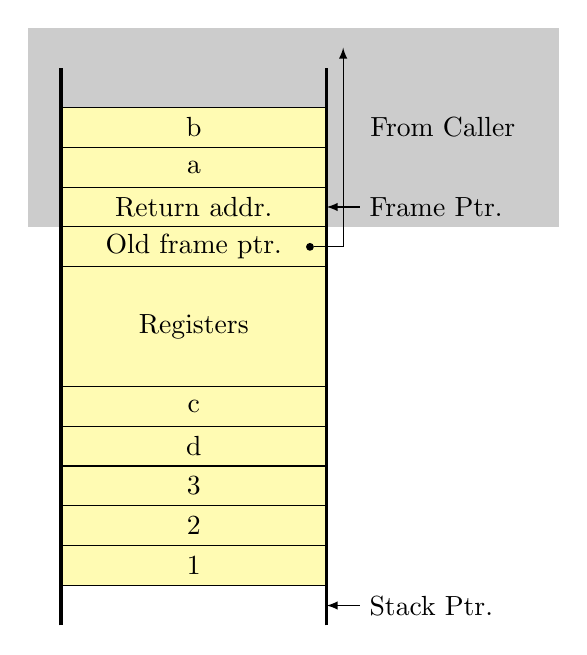
\begin{tikzpicture}[x=1pc,y=1.2pc]

\fill [fill=black!20] (-1,12) rectangle (15,17);
\node at (11.5,14.5) {From Caller};

\draw [thin,fill=yellow!30] (0,15) rectangle node {b} ++(8,-1);
\draw [thin,fill=yellow!30] (0,14) rectangle node {a} ++(8,-1);
\draw [thin,fill=yellow!30] (0,13) rectangle node {Return addr.} ++(8,-1);
\draw [thin,fill=yellow!30] (0,12) rectangle node {Old frame ptr.} ++(8,-1);
\node [fill,circle,inner sep=1pt] at (7.5,11.5) (ofp) {};
\draw [thin,fill=yellow!30] (0,11) rectangle node {Registers} ++(8,-3);
\draw [thin,fill=yellow!30] (0,8) rectangle node {c} ++(8,-1);
\draw [thin,fill=yellow!30] (0,7) rectangle node {d} ++(8,-1);
\draw [thin,fill=yellow!30] (0,6) rectangle node {3} ++(8,-1);
\draw [thin,fill=yellow!30] (0,5) rectangle node {2} ++(8,-1);
\draw [thin,fill=yellow!30] (0,4) rectangle node {1} ++(8,-1);

\draw [<-] (8,12.5) -- ++(right:1) node [right] {Frame Ptr.};
\draw [<-] (8,2.5) -- ++(right:1) node [right] {Stack Ptr.};

\draw [->] (ofp) -- ++(right:1) -- ++(up:5);

\draw [very thick] (0,2) -- (0,16);
\draw [very thick] (8,2) -- (8,16);
\end{tikzpicture}
\end{column}
\end{columns}
\end{frame}

\begin{frame}[fragile]{Recursive Fibonacci}

\begin{columns}
  \begin{column}{0.2\textwidth}
    (Real C)

    \begin{C}
int fib(int n) {

  if (n<2)

    return 1;
  else
    return
       fib(n-1)
       +
       fib(n-2);

}
\end{C}
  \end{column}
  \begin{column}{0.5\textwidth}
    (Assembly-like C)

\begin{C}
int fib(int n) {
    int tmp1, tmp2, tmp3;
    tmp1 = n < 2;
    if (!tmp1) goto L1;
    return 1;
L1: tmp1 = n - 1;
    tmp2 = fib(tmp1);
L2: tmp1 = n - 2;
    tmp3 = fib(tmp1);
L3: tmp1 = tmp2 + tmp3;
    return tmp1;
}
\end{C}
  \end{column}
\end{columns}

\begin{center}
\footnotesize
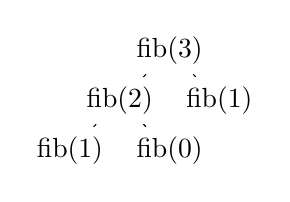
\begin{tikzpicture}
  \path [level distance=1.5pc]
  node {fib(3)}
    child [sibling distance=3pc] {node {fib(2)}
      child {node {fib(1)}}
      child {node {fib(0)}}
    }
    child [sibling distance=3pc] {node {fib(1)}}
  ;
\end{tikzpicture}
\includegraphics[width=0.3\textwidth]{russian-nesting-dolls.jpg}
\end{center}
\end{frame}

\def\mynode#1{\tikz[remember picture] \node (#1) {};}
\def\fp#1{
  \node [fill,circle,inner sep=1pt] at ($(#1.north east) + (-1pc,-19pt)$)
  (#1-fp) {};}
\def\ra#1{
  \node [fill,circle,inner sep=1pt] at ($(#1.north east) + (-1pc,-6pt)$)
  (#1-ra) {};}
\def\thefp#1{
  \node [arrow box, color=white, fill=gray, arrow box arrows={east:8pt},
         anchor=east]
  at ($(#1.north west) + (0,-6pt)$) {\sffamily \bfseries FP};
}
\def\thesp#1{
  \node [arrow box, color=white, fill=gray, arrow box arrows={east:8pt},
         anchor=east]
  at ($(#1.south west) + (0,-6pt)$) {\sffamily \bfseries SP};
}

\begin{frame}[fragile]{Executing fib(3)}

  \begin{columns}
    \begin{column}{0.5\textwidth}
      \begin{semiverbatim}
\hlta<2,3,4,6,9>int fib(int n) \{
    int tmp1, tmp2, tmp3;
    tmp1 = n < 2;
    if (!tmp1) goto L1;
\hlta<4,6,9>    return 1;
\hlta<2,3>L1: tmp1 = n - 1;
\hlta<5,8>    tmp2 = \hlta<2,3>fib(tmp1);\mynode{pc1}
\hlta<5,8>L2: tmp1 = n - 2;
\hlta<7,10>    tmp3 = \hlta<5,8>fib(tmp1);\mynode{pc2}
\hlta<7,10>L3: tmp1 = tmp2 + tmp3;
    return tmp1;
\}
      \end{semiverbatim}
%\only<1>{1}\only<2>{2}\only<3>{3}\only<4>{4}\only<5>{5}\only<6>{6}\only<7>{7}\only<8>{8}\only<9>{9}\only<10>{10}
    \end{column}
    \begin{column}{0.5\textwidth}
      \begin{overlayarea}{\textwidth}{\textheight}
        \small
      \begin{tikzpicture}[remember picture]
        \matrix [every node/.style={draw,fill=white,drop shadow,
            text width=8pc}] {
            \node [draw=white] (s0) {n = 3}; \\
            \only<2->{
            \node (s1) {return address\\
              last frame pointer \\
              tmp1 = \only<2-7>{2}%
                     \only<8-9>{1}%
                     \only<10>{3\textcolor{red}{$\leftarrow$ result}}\\
              tmp2 = \only<8->{2}\\
              tmp3 = \only<10>{1}
              \only<2-9>{\\
              n = \only<2-7>{2}%
                  \only<8->{1}}}; }\\
            \only<3-7,9>{
            \node (s2) {return address\\
              last frame pointer \\
              tmp1 = \only<3-4,9>{1}%
                     \only<5-6>{0}%
                     \only<7>{2}\\
              tmp2 = \only<5-7>{1}\\
              tmp3 = \only<7>{1}\\
              \only<1-6>{n = \only<1-4>{1}%
                  \only<5->{0}}}; } \\
            \only<4,6>{
            \node (s3) {return address\\
              last frame pointer \\
              tmp1 = 1\\
              tmp2 = \\
              tmp3 =}; } \\
        };
        \only<1>{\thesp{s0}}
        \only<2,8,10>{\thefp{s1}\thesp{s1}}
        \only<3,5,7,9>{\thefp{s2}\thesp{s2}}
        \only<4,6>{\thefp{s3}\thesp{s3}}
        \only<2->{\fp{s1}\ra{s1}}
        \only<3-7,9>{\fp{s2}\ra{s2}}
        \only<4,6>{\fp{s3}\ra{s3}}
        \draw (s0.north west) -- (s0.south west) --
              (s0.south east) -- (s0.north east);
      \end{tikzpicture}
      \end{overlayarea}
      \begin{tikzpicture}[remember picture, overlay]
        \only<2->{
          \draw [->] (s1-fp) -| ++(3pc,4pc);
          \draw [->] (s1-ra) -- ++ (-2pc,2pc);
        }
        \only<3-7>{
          \draw [->] (s2-ra) to [out=-150,in=10] (pc1);}
        \only<9>{
          \draw [->] (s2-ra) to [out=-150,in=10] (pc2);}
        \only<3-7,9>{
          \draw [->] (s2-fp) -- ++(4pc,0) |-
                ($(s1.north east)+(0,-6pt)$);
        }
        \only<4>{\draw [->] (s3-ra) to [out=150,in=-10] (pc1);}
        \only<6>{\draw [->] (s3-ra) to [out=150,in=-10] (pc2);}
        \only<4,6>{
          \draw [->] (s3-fp) -- ++(3pc,0) |-
                ($(s2.north east)+(0,-6pt)$);
        }
      \end{tikzpicture}
    \end{column}
  \end{columns}

\end{frame}

\begin{frame}[fragile]{Allocating Fixed-Size Arrays}

Local arrays with fixed size are easy to stack.

\begin{minipage}{0.3\textwidth}
\begin{C}
void foo()
{
  int a;
  int b[10];
  int c;
}
\end{C}
\end{minipage}
%
\begin{tabular}{|c|l}
\\
\cline{1-1}
return address & $\leftarrow$ FP \\
\cline{1-1}
a \\
\cline{1-1}
b[9] \\
$\vdots$ \\
b[0] \\
\cline{1-1}
c & $\leftarrow$ FP $-$ 48 \\
\cline{1-1}
\\
\end{tabular}

\end{frame}



\begin{frame}[fragile]
  \frametitle{Allocating Variable-Sized Arrays}

Variable-sized local arrays aren't as easy.

\begin{minipage}{0.37\textwidth}
\begin{C}
void foo(int n)
{
  int a;
  int b[n];
  int c;
}
\end{C}

\end{minipage}
%
\begin{tabular}{|c|l}
\\
\cline{1-1}
return address & $\leftarrow$ FP \\
\cline{1-1}
a \\
\cline{1-1}
b[n-1] \\
$\vdots$ \\
b[0] \\
\cline{1-1}
c & $\leftarrow$ FP $-$ ? \\
\cline{1-1}
\end{tabular}

Doesn't work: generated code expects a fixed offset for c.  Even worse 
for multi-dimensional arrays.

\end{frame}

\begin{frame}[fragile]
  \frametitle{Allocating Variable-Sized Arrays}

\begin{minipage}{0.5\textwidth}
As always:\\ add a level of indirection

\medskip

\begin{C}
void foo(int n)
{
  int a;
  int b[n];
  int c;
}
\end{C}
\end{minipage}
%
\begin{tabular}{|c|@{}l}
\\
\cline{1-1}
return address & $\leftarrow$ FP \\
\cline{1-1}
a \\
\cline{1-1}
\tikz[remember picture] \node (b) {b-ptr}; \\
\cline{1-1}
c \\
\cline{1-1}
b[n-1] \\
$\vdots$ \\
\tikz[remember picture] \node (b1) {b[0]}; \\[-3pt]
\cline{1-1}
\end{tabular}

\begin{tikzpicture}[remember picture,overlay]
  \draw [->] (b) to [out=-10,in=10] (b1);
\end{tikzpicture}

Variables remain constant offset from frame pointer.

\end{frame}




\begin{frame}[fragile]{Nesting Function Definitions}

\begin{columns}
  \begin{column}{0.5\textwidth}
\shadowstart
\begin{lstlisting}[language=caml,morendkeywords={words},ndkeywordstyle={\itshape\color{red}}]
let articles words =

  let report w =

    let count = List.length
      (List.filter ((=) w) words)
    in w ^ ": " ^
       string_of_int count

  in String.concat ", "
    (List.map report ["a"; "the"])

in articles
    ["the"; "plt"; "class"; "is";
     "a"; "pain"; "in";
     "the"; "butt"]
\end{lstlisting}
\shadowend
  \end{column}
  \begin{column}{0.5\textwidth}
\shadowstart
\begin{lstlisting}[language=caml,morendkeywords={words},ndkeywordstyle={\itshape\color{red}}]
let count words w = List.length
  (List.filter ((=) w) words) in

let report words w = w ^ ": " ^
  string_of_int (count words w) in

let articles words =
  String.concat ", "
    (List.map (report words)
     ["a"; "the"]) in

articles
    ["the"; "plt"; "class"; "is";
     "a"; "pain"; "in";
     "the"; "butt"]
\end{lstlisting}
\shadowend
  \end{column}
\end{columns}

Produces ``a: 1, the: 2''

\end{frame}

\def\stackframe#1#2{
 \node [frame] (#1) {(access link)\\#2}
    node [fill,circle,inner sep=1pt] at ($(#1.north east) + (-6pt,-6pt)$)
      (#1-sl) {}
    node [anchor=east] at (#1.west) {#1:};
}

\def\link#1#2{
  \draw [->] (#1-sl) to [out=45,in=-15] ($(#2.north east) + (0,-6pt)$);
}

\begin{frame}[fragile]{Implementing Nested Functions with Access Links}

\begin{columns}
  \begin{column}{0.5\textwidth}
\begin{ocaml}
let a x s =

  let b y =

    let c z = z + s in

    let d w = c (w+1) in

    d (y+1) in (* b *)

  let e q = b (q+1) in

e (x+1) (* a *)
\end{ocaml}

What does ``a 5 42'' give?

% 51

  \end{column}
  \begin{column}{0.5\textwidth}
      \begin{overlayarea}{\textwidth}{0.8\textheight}
\begin{tikzpicture}
  \matrix [frame/.style={draw,fill=white,drop shadow,text width=6pc},
           row sep=5pt] {
    \stackframe{a}{x = 5\\s = 42} \\
    \only<2->{\stackframe{e}{q = 6}} \\
    \only<3->{\stackframe{b}{y = 7}} \\
    \only<4->{\stackframe{d}{w = 8}} \\
    \only<5->{\stackframe{c}{z = 9}} \\
    };
  \only<2->{\link e a}
  \only<3->{\link b a}
  \only<4->{\link d b}
  \only<5->{\link c b}
\end{tikzpicture}
      \end{overlayarea}
  \end{column}
\end{columns}
\end{frame}

\subsection{In-Memory Layout Issues}

\begin{frame}[fragile]{Layout of Records and Unions}

Modern processors have byte-addressable memory.

\begin{columns}
  \begin{column}{0.1\textwidth}
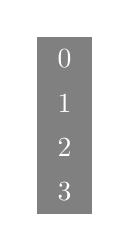
\begin{tikzpicture}
  \matrix [every node/.style=byte] {
    \node {0}; \\
    \node {1}; \\
    \node {2}; \\
    \node {3}; \\
  };
\end{tikzpicture}
  \end{column}
  \begin{column}{0.35\textwidth}
    \includegraphics[width=\textwidth]{ibm_360.jpg}
  \end{column}
  \begin{column}{0.4\textwidth}   
    \small The IBM 360 (c. 1964) helped to popularize byte-addressable memory.
  \end{column}
\end{columns}

Many data types (integers, addresses, floating-point numbers) are
wider than a byte.

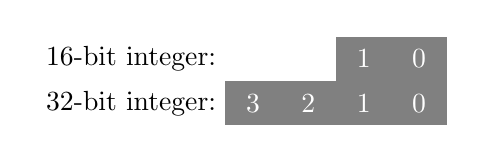
\begin{tikzpicture}
  \matrix {
    \node {16-bit integer:}; & & & \node [byte] {1}; & \node [byte] {0}; \\
    \node {32-bit integer:}; & \node [byte] {3}; & \node [byte] {2}; &
                            \node [byte] {1}; & \node [byte] {0}; \\
    };
\end{tikzpicture}
\hspace{3pc}
\includegraphics[width=4pc]{byte-me-candy-heart.jpg}

\end{frame}



\begin{frame}[fragile]{Layout of Records and Unions}

\begin{columns}
  \begin{column}{0.5\textwidth}
\parskip=6pt

Modern memory systems read data in 32-, 64-, or 128-bit chunks:

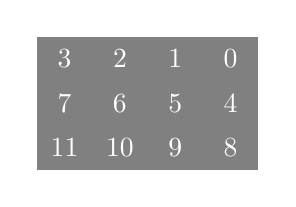
\begin{tikzpicture}
  \matrix [every node/.style=byte] {
     \node {3}; &  \node {2}; & \node {1}; & \node {0}; \\
     \node {7}; &  \node {6}; & \node {5}; & \node {4}; \\
    \node {11}; & \node {10}; & \node {9}; & \node {8}; \\
    };
\end{tikzpicture}

Reading an aligned 32-bit value is fast: a single operation.

\begin{tikzpicture}
  \matrix [every node/.style=byte] {
     \node {3}; &  \node {2}; & \node {1}; & \node {0}; \\
     \node [hbyte] {7}; & \node [hbyte] {6}; & \node [hbyte] {5}; & \node [hbyte] {4}; \\
    \node {11}; & \node {10}; & \node {9}; & \node {8}; \\
    };
\end{tikzpicture}
  \end{column}
  \begin{column}{0.5\textwidth}
\parskip=6pt

    It is harder to read an unaligned value: two reads plus shifting

\begin{tikzpicture}
  \matrix [every node/.style=byte] {
     \node [hbyte] (3) {3}; &  \node {2}; & \node {1}; & \node {0}; \\
     \node {7}; & \node [hbyte] (6) {6}; & \node [hbyte] (5) {5}; & \node [hbyte] (4) {4}; \\
    \node {11}; & \node {10}; & \node {9}; & \node {8}; \\
    \\[15pt]
     \node [hbyte] (6a) {6}; & \node [hbyte] (5a) {5}; & \node [hbyte] (4a) {4}; & \node [hbyte] (3a) {3}; \\
    };
  \draw [->] (3) edge (3a)
             (4) edge (4a)
             (5) edge (5a)
             (6) edge (6a);
\end{tikzpicture}

SPARC and ARM prohibit unaligned accesses

MIPS has special unaligned load/store instructions

x86, 68k run more slowly with unaligned accesses

  \end{column}
\end{columns}
\end{frame}

\begin{frame}[fragile]{Padding}

To avoid unaligned accesses, the C compiler pads the layout of unions
and records.

Rules:

\begin{itemize}
  \item Each $n$-byte object must start on a multiple of $n$ bytes (no
    unaligned accesses).

   \item Any object containing an $n$-byte object must be of size $mn$ for some
     integer $m$ (aligned even when arrayed).
\end{itemize}

\begin{columns}
  \begin{column}[t]{0.5\textwidth}
\begin{C}
struct padded {
  int x;   /* 4 bytes */
  char z;  /* 1 byte  */
  short y; /* 2 bytes */
  char w;  /* 1 byte  */
};
\end{C}

\begin{tikzpicture}
  \matrix [every node/.style=hbyte] {
    \node {x}; & \node {x}; & \node {x}; & \node {x}; \\
    \node {y}; & \node {y}; & \node [byte] {}; & \node {z}; \\
    \node [byte] {}; & \node [byte] {}; & \node [byte] {}; & \node {w}; \\
    };
\end{tikzpicture}
  \end{column}
  \begin{column}[t]{0.5\textwidth}
\begin{C}
struct padded {
  char a;  /* 1 byte  */
  short b; /* 2 bytes */
  short c; /* 2 bytes */
};
\end{C}

\begin{tikzpicture}
  \matrix [every node/.style=hbyte] {
    \node {b}; & \node {b}; & \node [byte] {}; & \node {a}; \\
     & & \node {c}; & \node {c}; \\
    };
\end{tikzpicture}
  \end{column}
\end{columns}

\end{frame}

\begin{frame}[fragile]{Unions}

A C \emph{struct} has a separate space for each field; a C
\emph{union} shares one space among all fields

\begin{columns}
  \begin{column}[t]{0.5\textwidth}
\begin{C}
union intchar {
  int i;   /* 4 bytes */
  char c;  /* 1 byte  */
};
\end{C}

\begin{tikzpicture}
  \matrix [every node/.style=hbyte] {
    \node {i}; & \node {i}; & \node {i}; & \node {i/c}; \\
    };
\end{tikzpicture}
  \end{column}
  \begin{column}[t]{0.5\textwidth}
\begin{C}
union twostructs {
  struct {
    char c;   /* 1 byte */
    int i;    /* 4 bytes */
  } a;
  struct {
    short s1; /* 2 bytes */
    short s2; /* 2 bytes */
  } b;
};
\end{C}

\begin{tikzpicture}
  \matrix [every node/.style=hbyte] at (0,2pc) {
    \node [byte] {}; &
    \node [byte] {}; &
    \node [byte] {}; &
    \node {c}; \\
    \node {i}; &
    \node {i}; &
    \node {i}; &
    \node {i}; \\
  };

\node {or};

  \matrix [every node/.style=hbyte] at (0,-2pc) {
    \node {s2}; &
    \node {s2}; &
    \node {s1}; &
    \node {s1}; \\
    \node [byte] {}; &
    \node [byte] {}; &
    \node [byte] {}; &
    \node [byte] {}; \\
  };
\end{tikzpicture}
  \end{column}
\end{columns}

\end{frame}

\begin{frame}[t,fragile]{Arrays}

\makebox[\textwidth][r]{\raisebox{-2pc}[0pt][0pt]{%
  \includegraphics[width=0.35\textwidth]{ospedale-delgi-innocenti.jpg}}}

\vspace{2pc}

\begin{columns}
  \begin{column}{0.5\textwidth}
Basic policy in C: an array is just one
object after another in memory.

\medskip

\begin{C}
int a[10];
\end{C}
  \end{column}
  \begin{column}{0.5\textwidth}
\begin{tikzpicture}
  \matrix [bytes] {
    a[0] & a[0] & a[0] & a[0] \\
    a[1] & a[1] & a[1] & a[1] \\[1.5pc]
    a[9] & a[9] & a[9] & a[9] \\
  };
\node at (0,-0.5pc) {$\vdots$};
\end{tikzpicture}
  \end{column}
\end{columns}

\vspace{1pc}

\begin{columns}
  \begin{column}{0.5\textwidth}
This is why you need padding at the end of \emph{structs}.

\medskip

\begin{C}
struct {
  int a;
  char c;
} b[2];
\end{C}
  \end{column}
  \begin{column}{0.5\textwidth}
\begin{tikzpicture}
  \matrix [bytes] (bytes) {
    a & a & a & a \\
    & & & c \\
    a & a & a & a \\
    & & & c \\
  };
\node [right] at ($(bytes.north east)!0.25!(bytes.south east)$) {b[0]};
\node [right] at ($(bytes.north east)!0.75!(bytes.south east)$) {b[1]};
\end{tikzpicture}
  \end{column}
\end{columns}

\end{frame}

\begin{frame}[fragile]{Arrays and Aggregate types}

\begin{columns}
  \begin{column}{0.5\textwidth}
The largest primitive type dictates the alignment

\medskip

\begin{C}
struct {
  short a;
  short b;
  char c;
} d[4];
\end{C}
  \end{column}
  \begin{column}{0.5\textwidth}
\begin{tikzpicture}
  \matrix [bytes] (bytes) {
    b & b & a & a \\
    a & a &   & c \\
      & c & b & b \\
    b & b & a & a \\
    a & a &   & c \\
      & c & b & b \\
  };
\node [right] at ($(bytes.north east)!0.0833!(bytes.south east)$) {d[0]};
\node [right] at ($(bytes.north east)!0.25!(bytes.south east)$) {d[1]};
\node [right] at ($(bytes.north east)!0.583!(bytes.south east)$) {d[2]};
\node [right] at ($(bytes.north east)!0.75!(bytes.south east)$) {d[3]};
\end{tikzpicture}
  \end{column}
\end{columns}

\end{frame}

\begin{frame}[fragile]{Arrays of Arrays}
\begin{columns}
  \begin{column}{0.3\textwidth}
\begin{C}
char a[4];
\end{C}
  \end{column}
  \begin{column}{0.7\textwidth}
\begin{tikzpicture}
  \matrix [bytes] (bytes) {
    a[3] & a[2] & a[1] & a[0] \\
  };
\end{tikzpicture}
  \end{column}
\end{columns}

\vspace{3pc}

\begin{columns}
  \begin{column}{0.3\textwidth}
\begin{C}
char a[3][4];
\end{C}
  \end{column}
  \begin{column}{0.7\textwidth}
\begin{tikzpicture}
  \matrix [bytes] (bytes) {
    a[0][3] & a[0][2] & a[0][1] & a[0][0] \\
    a[1][3] & a[1][2] & a[1][1] & a[1][0] \\
    a[2][3] & a[2][2] & a[2][1] & a[2][0] \\
  };
\node [right] at ($(bytes.north east)!0.166!(bytes.south east)$) {a[0]};
\node [right] at ($(bytes.north east)!0.5!(bytes.south east)$) {a[1]};
\node [right] at ($(bytes.north east)!0.833!(bytes.south east)$) {a[2]};
\end{tikzpicture}
  \end{column}
\end{columns}
\end{frame}

\subsection{The Heap}

\begin{frame}
  \frametitle{Heap-Allocated Storage}

Static works when you know everything beforehand and always need it.

Stack enables, but also requires, recursive behavior.

A \emph{heap} is a region of memory where blocks can be allocated and
deallocated in any order.

(These heaps are different than those in, e.g., heapsort)

\end{frame}



\begin{frame}[fragile]
  \frametitle{Dynamic Storage Allocation in C}

\shadowstart
\begin{lstlisting}[language=C,morendkeywords={malloc,free},ndkeywordstyle={\itshape\color{red}}]
struct point {
   int x, y;
};

int play_with_points(int n)
{
  int i;
  struct point *points;

  points = malloc(n * sizeof(struct point));

  for ( i = 0 ; i < n ; i++ ) {
    points[i].x = random();
    points[i].y = random();
  }

  /* do something with the array */

  free(points);
}
\end{lstlisting}
\shadowend

\end{frame}

\newlength{\unitbox}
\setlength{\unitbox}{3.5em}
\newcommand{\used}[1]{%
\tikz[baseline=-3pt] \node [used, minimum width=#1\unitbox] {};}

\newcommand{\free}[1]{%
\tikz[baseline=-3pt] \node [free, minimum width=#1\unitbox] {};}

\begin{frame}
  \frametitle{Dynamic Storage Allocation}

\parskip=1pc

\used{1}\used{2}\free{1}\used{2.5}\free{0.5}\used{0.5}\used{0.2}

\pause

\hspace{\unitbox}\hbox to 2\unitbox{\hfil $\downarrow$\rlap{ \texttt{free(\used{2})}} \hfil}

\pause

\used{1}\free{3}\used{2.5}\free{0.5}\used{0.5}\used{0.2}

\pause

\hspace{1.5\unitbox}$\downarrow$ \texttt{malloc(\used{2.5})}

\pause

\used{1}\used{2.5}\free{0.5}\used{2.5}\free{0.5}\used{0.5}\used{0.2}

\end{frame}



\begin{frame}
  \frametitle{Dynamic Storage Allocation}

Rules:

{\parindent=1em
Each allocated block contiguous (no holes)

Blocks stay fixed once allocated
}

\texttt{malloc()}

{\parindent=1em
Find an area large enough for requested block

Mark memory as allocated
}

\texttt{free()}

{\parindent=1em
Mark the block as unallocated
}

\makebox[\textwidth][r]{\raisebox{-2pc}[0pt][0pt]{%
  \includegraphics[width=10pc]{sushi-conveyor-restaurant.jpg}}}

\end{frame}


\begin{frame}
  \frametitle{Simple Dynamic Storage Allocation}

Maintaining information about free memory

{\parindent=1em
Simplest: Linked list
}

The algorithm for locating a suitable block

{\parindent=1em
Simplest: First-fit
}

The algorithm for freeing an allocated block

{\parindent=1em
Simplest: Coalesce adjacent free blocks
}

\end{frame}

\setlength{\unitbox}{1.3pc}

\begin{frame}[fragile]{Simple Dynamic Storage Allocation}

  \begin{tikzpicture}[node distance=1pc]
    \matrix (m0) {
      \node [free,minimum width=1\unitbox] {S}; &
      \node [free,minimum width=1\unitbox] (n0) {N}; &
      \node [free,minimum width=5\unitbox] {}; &
      \node [used,minimum width=1\unitbox] {S}; &
      \node [used,minimum width=2\unitbox] {}; &
      \node [free,minimum width=1\unitbox] {S}; &
      \node [free,minimum width=1\unitbox] (n1) {N}; &
      \node [free,minimum width=2\unitbox] {};
      \\
    };
    \draw [<-] (n0.north) to [out=135,in=0] ($(n0.north) + (-3pc,1pc)$);
    \draw [->] (n0.north) .. controls ($(n0.north) + (1pc,2pc)$) and
    ($(n1.north) + (-1pc,2pc)$) .. (n1.north);
    \draw [->] (n1.north) to [out=45,in=180] ($(n1.north) + (4pc,1pc)$);

    \pause

    \matrix [below=of m0] (m1) {
      \node {\ttfamily malloc(}; &
      \node [used,minimum width=3\unitbox] {}; &
      \node {\ttfamily )}; \\
    };

    \pause

    \matrix [below=of m1] (m2) {
      \node [used,minimum width=1\unitbox] {S}; &
      \node [used,minimum width=3\unitbox]  {}; &
      \node [free,minimum width=1\unitbox] {S}; &
      \node [free,minimum width=1\unitbox] (n2) {N}; &
      \node [free,minimum width=1\unitbox] {}; &
      \node [used,minimum width=1\unitbox] {S}; &
      \node [used,minimum width=2\unitbox] (u0) {}; &
      \node [free,minimum width=1\unitbox] {S}; &
      \node [free,minimum width=1\unitbox] (n3) {N}; &
      \node [free,minimum width=2\unitbox] {};
      \\
    };

    \draw [<-] (n2.north) to [out=145,in=0] ($(n2.north) + (-8pc,1pc)$);
    \draw [->] (n2.north) .. controls ($(n2.north) + (1pc,1.5pc)$) and
    ($(n3.north) + (-1pc,1.5pc)$) .. (n3.north);
    \draw [->] (n3.north) to [out=45,in=180] ($(n3.north) + (4pc,1pc)$);

    \pause

    \matrix [below=of m2] (m3) {
      \node {\ttfamily free(}; &
      \node [fill,circle,inner sep=1pt] at (0,-6pt) (p1) {}; & 
      \node {\ttfamily )}; \\
    };

    \draw [->] (p1) to [out=80,in=-100] (u0.south west);

    \pause 

    \matrix [below=of m3] (m4) {
      \node [used,minimum width=1\unitbox] {S}; &
      \node [used,minimum width=3\unitbox]  {}; &
      \node [free,minimum width=1\unitbox] {S}; &
      \node [free,minimum width=1\unitbox] (n4) {N}; &
      \node [free,minimum width=8\unitbox] {};
      \\
    };

    \draw [<-] (n4.north) to [out=145,in=0] ($(n4.north) + (-8pc,1pc)$);
    \draw [->] (n4.north) to [out=35,in=180] ($(n4.north) + (12pc,1pc)$);

  \end{tikzpicture}

\end{frame}

\begin{frame}{Fragmentation}

\texttt{malloc( \used{2} )} seven times give

\used{2}\used{2}\used{2}\used{2}\used{2}\used{2}\used{2}

\medskip

\texttt{free()} four times gives

\free{2}\used{2}\free{2}\used{2}\free{2}\used{2}\free{2}

\medskip

\texttt{malloc( \used{4} )} ?

Need more memory; can't use fragmented memory.

\begin{tabular}{cc}
  \includegraphics[height=5pc]{Zebra.jpg}
  &
  \includegraphics[height=4.5pc]{Tapir.jpg}
  \\
  Zebra
  &
  Tapir
  \\
\end{tabular}

\end{frame}

\begin{frame}[fragile]{Fragmentation and Handles}

Standard CS solution: Add another layer of indirection.

Always reference memory through ``handles.''

\begin{columns}
  \begin{column}{0.7\textwidth}
\begin{overlayarea}{\textwidth}{2pc}
\begin{tikzpicture}[node distance=2pc]

  \matrix (m0) {
  \only<1>{
    \node [free,minimum width=2\unitbox] {}; &
    \node [used,minimum width=2\unitbox] (u0) {}; &
    \node [free,minimum width=2\unitbox] {}; &
    \node [used,minimum width=2\unitbox] (u1) {}; &
    \node [free,minimum width=2\unitbox] {}; &
    \node [used,minimum width=2\unitbox] (u2) {};
  }%
  \only<2>{
    \node [used,minimum width=2\unitbox] (u0) {}; &
    \node [used,minimum width=2\unitbox] (u1) {}; &
    \node [used,minimum width=2\unitbox] (u2) {}; &
    \node [free,minimum width=6\unitbox] {};
  }%
    \\
  };

  \matrix [below=of m0.south west,anchor=base,matrix anchor=north west] (m1) {
    \node (pa) {\ttfamily *a}; &
    \node (pb) {\ttfamily *b}; &
    \node (pc) {\ttfamily *c}; &
    \node {Pointers}; \\
  };

  \matrix [below=of m1,anchor=base] (m2) {
    \node (ha) {\ttfamily **a}; &
    \node (hb) {\ttfamily **b}; &
    \node (hc) {\ttfamily **c}; &
    \node {Handles}; \\
  };

  \draw [->] (ha) -- (pa);
  \draw [->] (pa) -- (u0.south west);
  \draw [->] (hb) -- (pb);
  \draw [->] (pb) -- (u1.south west);
  \draw [->] (hc) -- (pc);
  \draw [->] (pc) -- (u2.south west);

\end{tikzpicture}
\end{overlayarea}
  \end{column}
  \begin{column}{0.3\textwidth}
    \includegraphics[width=\textwidth]{apple_1984_mac.jpg}

    \raggedright
    The original Macintosh did this to save memory.
  \end{column}
\end{columns}

\end{frame}

\subsection{Automatic Garbage Collection}

\begin{frame}{Automatic Garbage Collection}

Entrust the runtime system with freeing heap objects

Now common: Java, C\#, Javascript, Python, Ruby, OCaml and most
functional languages

\medskip

\begin{columns}[t]
\begin{column}{0.5\textwidth}
\parskip=0.5\baselineskip
\textbf{Advantages}

Much easier for the programmer

Greatly improves reliability: no memory leaks, double-freeing, or
other memory management errors
\end{column}
\begin{column}{0.5\textwidth}
\parskip=0.5\baselineskip
\textbf{Disadvantages}

Slower, sometimes unpredictably so

May consume more memory

\includegraphics[width=\textwidth]{garbage-truck.jpg}

\end{column}
\end{columns}

\end{frame}

\begin{frame}[fragile,t]{Reference Counting}

What and when to free? 

\begin{itemize}
\item Maintain count of references to each object
\item Free when count reaches zero
\end{itemize}

\begin{columns}[t]
\begin{column}{0.4\textwidth}
\begin{semiverbatim}
\hlta<2>let a = \hlta<1>(42, 17) in
\hlta<4>let b = \hlta<3>[a;a] in
\hlta<6>let c = \hlta<5>(1,2)::b in
\hlta<7-10>b
\end{semiverbatim}
\end{column}
\begin{column}{0.6\textwidth}
\ttfamily

\begin{tikzpicture}[cell/.style={rectangle split,
      rectangle split horizontal, fill=white, draw,
      anchor=west}]
\fill [color=yellow!30] (-6pc,2.5pc) rectangle (9pc,-10pc);
\node [cell, rectangle split parts=2]
      (aa) {\only<1>{0}%
            \only<2>{1}%
            \only<3-6>{3}%
            \only<7->{2}%
            \nodepart{two} 42, 17};
\only<2-6>{
  \node (a) at ($(aa) + (-3pc, 2pc)$) {a};
  \draw [->] (a) to [bend left] (aa);
}
\only<3->{
  \node [cell, rectangle split parts=3] (bb)
      at ($(aa.west) + (down:3pc)$)
      {\only<3>{0}%
       \only<4,9->{1}%
       \only<5-8>{2}%
       \nodepart{two} \nodepart{three}};
  \node [cell, rectangle split parts=3] (bbb)
      at ($(bb.east) + (right:2pc)$)
      {1 \nodepart{two} \nodepart{three}};
  \draw [->] (bb.two) to (aa);
  \draw [->] (bb.three) to (bbb);
  \draw [->] (bbb.two) to [bend right] (aa);
  \draw [-open triangle 90] (bbb.three) -| ++(1pc,-1pc);
}
\only<4-10>{
  \node (b) at ($(bb) + (-2pc,1.5pc)$) {b};
  \draw [->] (b) to [bend left] (bb);
}
\only<5-9>{
  \node [cell, rectangle split parts=2] (ccc) at ($(bb.west) + (-5pc,-3pc)$) 
        {\only<5-8>{1}%
         \only<9>{0}%
         \nodepart{two} 1, 2};
}
\only<5-8>{
  \node [cell, rectangle split parts=3] (cc) at ($(bb) + (-6pc,0)$)
        {\only<5,8>{0}%
         \only<6-7>{1}%
         \nodepart{two} \nodepart{three}};
  \draw [->] (cc.two) to (ccc);
  \draw [->] (cc.three) to (bb);
}
\only<6-7>{
  \node (c) at ($(cc) + (-1pc,2pc)$) {c};
  \draw [->] (c) to [bend left] (cc);
}
\end{tikzpicture}

\end{column}
\end{columns}

\end{frame}

\begin{frame}{Issues with Reference Counting}

Circular structures defy reference counting:

\begin{tikzpicture}
  \node [draw] (a) {a};
  \node [draw,right=of a] (b) {b};
  \draw [->] (a) edge [bend left] (b);
  \draw [->] (b) edge [bend left] (a);
\end{tikzpicture}

Neither is reachable, yet both have non-zero reference counts.

High overhead (must update counts constantly), although incremental

\end{frame}

\begin{frame}[fragile,t]{Mark-and-Sweep}

What and when to free?

\begin{itemize}
\item Stop-the-world algorithm invoked when memory full
\item Breadth-first-search marks all reachable memory
\item All unmarked items freed
\end{itemize}

\begin{columns}[t]
\begin{column}{0.4\textwidth}
\begin{semiverbatim}
let a = (42, 17) in
let b = [a;a] in
let c = (1,2)::b in
b
\end{semiverbatim}
\end{column}
\begin{column}{0.6\textwidth}
\ttfamily

\begin{tikzpicture}[cell/.style={rectangle split,
      rectangle split horizontal, fill=white, draw,
      anchor=west}]
\fill [color=yellow!30] (-6pc,2.5pc) rectangle (9pc,-10pc);
\only<1-4>{
\node [cell, rectangle split parts=2]
      (aa) {\only<3>{$\bullet$}
            \nodepart{two} 42, 17};
}
\only<1>{
  \node (a) at ($(aa) + (-3pc, 2pc)$) {a};
  \draw [->] (a) to [bend left] (aa);
}
  \node [cell, rectangle split parts=3] (bb)
      at ($(aa.west) + (down:3pc)$)
      {\only<2-3>{$\bullet$}\nodepart{two} \nodepart{three}};
  \node [cell, rectangle split parts=3] (bbb)
      at ($(bb.east) + (right:2pc)$)
      { \only<3>{$\bullet$}\nodepart{two} \nodepart{three}};
  \draw [->] (bb.two) to (aa);
  \draw [->] (bb.three) to (bbb);
  \draw [->] (bbb.two) to [bend right] (aa);
  \draw [-open triangle 90] (bbb.three) -| ++(1pc,-1pc);
  \node (b) at ($(bb) + (-2pc,1.5pc)$) {b};
  \draw [->] (b) to [bend left] (bb);
\only<1-3>{
  \node [cell, rectangle split parts=2] (ccc) at ($(bb.west) + (-5pc,-3pc)$) 
        {\nodepart{two} 1, 2};
  \node [cell, rectangle split parts=3] (cc) at ($(bb) + (-6pc,0)$)
        {\nodepart{two} \nodepart{three}};
  \draw [->] (cc.two) to (ccc);
  \draw [->] (cc.three) to (bb);
}
\only<1>{
  \node (c) at ($(cc) + (-1pc,2pc)$) {c};
  \draw [->] (c) to [bend left] (cc);
}
\end{tikzpicture}

\end{column}
\end{columns}

\end{frame}

\begin{frame}{Mark-and-Sweep}
\parskip=0.5\baselineskip

Mark-and-sweep is faster overall; may induce big pauses

Mark-and-compact variant also moves or copies reachable objects to
eliminate fragmentation

Incremental garbage collectors try to avoid doing everything at once

Most objects die young; generational garbage collectors segregate heap
objects by age

Parallel garbage collection tricky

Real-time garbage collection tricky

\end{frame}

\subsection{Objects and Inheritance}

\begin{frame}[fragile]{Single Inheritance}

Simple: Add new fields to end of the object

Fields in base class always at same offset in derived class (compiler
never reorders)

Consequence: Derived classes can never remove fields

\vskip 2\baselineskip

\begin{columns}
\begin{column}[t]{0.5\textwidth}
\textbf{C++}

\begin{cpp}
class Shape {
  double x, y;
};

class Box : Shape {
  double h, w;
};


class Circle : Shape {
  double r;
};

\end{cpp}
\end{column}
\begin{column}[t]{0.5\textwidth}
\textbf{Equivalent C}

\begin{C}
struct Shape {
  double x, y;
};

struct Box {
  double x, y;
  double h, w;
};

struct Circle {
  double x, y;
  double r;
};
\end{C}
\end{column}
\end{columns}
\end{frame}

\begin{frame}[fragile]{Virtual Functions}

\begin{cpp}
class Shape {
  virtual void draw(); // Invoked by object's run-time class
};                     // not its compile-time type.

class Line : public Shape {
  void draw();
}

class Arc : public Shape {
  void draw();
};

Shape *s[10];
s[0] = new Line;
s[1] = new Arc;
s[0]->draw();   // Invoke Line::draw()
s[1]->draw();   // Invoke Arc::draw()
\end{cpp}

\end{frame}

\begin{frame}[fragile]{Virtual Functions}

Trick: add to each object a pointer to the virtual table for its type,
filled with pointers to the virtual functions.

Like the objects themselves, the virtual table for each derived type
begins identically.

\begin{columns}
\begin{column}{0.5\textwidth}
\begin{cpp}
struct A {
  int x;
  virtual void Foo();
  virtual void Bar();
};

struct B : A {
  int y;
  virtual void Foo();
  virtual void Baz();
};

A a1;
A a2;
B b1;
\end{cpp}
\end{column}
\begin{column}{0.5\textwidth}
\begin{tikzpicture}[%
  show background rectangle,
  background rectangle/.style={fill, color=yellow!30},
  object/.style={rectangle split,
                 fill=white,
                 draw
  }
]
\node [object, rectangle split parts=2] (Avtbl) {
   A::Foo
   \nodepart{two} A::Bar
   };
\node [above] at (Avtbl.north) {A's Vtbl};
\node [object, rectangle split parts=3, anchor=north] (Bvtbl)
   at ($(Avtbl.north) + (right:6pc)$) {
   B::Foo
   \nodepart{two} A::Bar
   \nodepart{three} B::Baz
   };
\node [above] at (Bvtbl.north) {B's Vtbl};

\node [object, rectangle split parts=2, anchor=north] (a1)
   at ($(Avtbl.south) + (down:2pc)$) { vptr
    \nodepart{second} x};
\node [above] at (a1.north) {a1};
\draw [->] (a1.text east) to [bend right] (Avtbl.text east);

\node [object, rectangle split parts=2, anchor=north] (a2)
   at ($(a1.south) + (down:2pc)$) { vptr
    \nodepart{second} x};
\node [above] at (a2.north) {a2};
\draw [->] (a2.text east) to [bend right] (Avtbl.text east);

\node [object, rectangle split parts=3, anchor=north] (b1)
   at ($(Bvtbl.south) + (down:2pc)$) { vptr
    \nodepart{second} x
    \nodepart{third} y
    };
\node [above] at (b1.north) {b1};
\draw [->] (b1.text east) to [bend right] (Bvtbl.text east);


   
\end{tikzpicture}
\end{column}
\end{columns}

\end{frame}

\subsection{Exceptions}

\def\mynode#1#2{\tikz[remember picture,baseline]\node[inner sep=0pt,anchor=base] (#1) {#2};}

\begin{frame}[fragile]{C++'s Exceptions}

\lstset{escapechar=\^}
\begin{cpp}
struct Except {} ex;  // This struct functions as an exception

void top(void) {
  try {
    ^\mynode{a}{child}^();
  } ^\mynode{f}{\bfseries catch}^ (Except e) { // throw sends control here
    printf("oops\n");
  }
}

void ^\mynode{b}{child}^() {
  ^\mynode{c}{child2}^();
}

void ^\mynode{d}{child2}^() {
  ^\mynode{e}{\textbf{throw} ex;}^ // Pass control up to the catch block
}
\end{cpp}

\begin{tikzpicture}[remember picture,overlay]
\begin{scope}[very thick, red, ->, font={\scriptsize},
              every node/.style={inner sep=2pt,draw,fill=white}]
\draw (a.south west) to [bend right=20] node [pos=0.7] {1} (b.north west);
\draw (c) to node [pos=0.35] {2} (d);
\draw [blue] (e.north east) to [bend right=55,looseness=1.5]
                            node [pos=0.25] {3} (f.south east);
\end{scope}
\end{tikzpicture}

\end{frame}

\begin{frame}[fragile]{C's setjmp/longjmp: Idiosyncratic Exceptions}

\vskip0.5\baselineskip

\lstset{escapechar=\^}
\begin{C}
#include <setjmp.h>

jmp_buf closure;          /* return address, stack & frame ptrs. */

void top(void) {
  switch ( ^\mynode{a}{setjmp}^(closure) ) { /* normal: store closure, return 0 */
                               /* longjmp jumps here, returns 1 */


  case 0: ^\mynode{b}{child}^();             /* unexceptional case */
          break;

  case 1: ^\mynode{e}{\bfseries break}^;               /* longjmp( ,1) called */
  }
}

void child() {
  ^\mynode{c}{child2}^();
}

void child2() {
  ^\mynode{d}{longjmp(closure, 1)}^;
}
\end{C}

\begin{tikzpicture}[remember picture,overlay]
\begin{scope}[very thick, red, ->, font={\scriptsize},
              every node/.style={inner sep=2pt,draw,fill=white}]
\draw (a.south) to node [pos=0.3] {1} (b.north);
\draw (b.south west) to [bend right=20] node [pos=0.15] {2} (c);
\draw (c) to node [pos=0.4] {3} ($(d.north west) + (right:1pc)$);
\draw [blue] (d.north east) to [bend right=60] node [pos=0.25] {4} (a.south east);
\draw [blue] (a.south east) to [bend left=45] node [pos=0.25] {5} (e.north east);
\end{scope}
\end{tikzpicture}

\end{frame}

\begin{frame}[fragile]{Implementing Exceptions}

One way: maintain a stack of exception handlers

\begin{columns}
\begin{column}{0.25\textwidth}
\begin{cpp}
try {

  child();


} catch (Ex e) {
  foo();
}

void child() {
  child2();
}

void child2() {
  throw ex;
}
\end{cpp}
\end{column}
\begin{column}{0.75\textwidth}
\begin{cpp}
  push(Ex, Handler); // Push handler on stack

  child();
  pop();             // Normal termination
  goto Exit;         // Jump over "catch"
Handler:
  foo();             // Body of "catch"
Exit:

void child() {
  child2();
}

void child2() {
  throw(ex);       // Unroll stack; find handler
}
\end{cpp}
\end{column}
\end{columns}

Incurs overhead, even when no exceptions thrown
\end{frame}

\begin{frame}[fragile]{Implementing Exceptions with Tables}

Q: When an exception is \emph{throw}n, where was the last \emph{try}?

A: Consult a table: relevant handler or ``pop'' for every PC

\begin{columns}
\begin{column}{0.4\textwidth}
\lstset{numbers=left,escapechar=\^}
\begin{cpp}
void foo() {

  try {
    ^\mynode{e}{bar();}^
  } catch (Ex1 e) {
    ^\mynode{g}{a();}^
  }
}

void bar() {
  ^\mynode{c}{baz();}^
}

void baz() {

  try {
    ^\mynode{a}{\textbf{throw} ex1;}^
  } catch (Ex2 e) {
    b();
  }
}
\end{cpp}
\end{column}
\begin{column}{0.5\textwidth}
%\renewcommand\arraystretch{2.3}
\begin{tabular}{rl}
\toprule
\textbf{Lines} & \textbf{Action} \\
\midrule
1--2 & Pop stack \\
\mynode{f}{3--5} & Handler @ 5 for Ex1 \\
\\
\\
\\
\mynode{d}{6--15} & Pop stack \\
\\
\\
\\
\mynode{b}{16--18} & Handler @ 14 for Ex2\\
\\
19--21 & Pop stack \\
\bottomrule
\end{tabular}

\end{column}
\end{columns}

\begin{tikzpicture}[remember picture,overlay]
\begin{scope}[very thick, red, ->, font={\scriptsize},
              every node/.style={inner sep=2pt,draw,fill=white}]
\draw (a.east) to node {1: query} (b.west);
\draw (b.west) to node [pos=0.4] {2: pop stack} (c.east);
\draw (c.east) to node {3: query} (d.west);
\draw (d.west) to node [pos=0.25] {4: pop stack} (e.east);
\draw (e.east) to [bend left=20] node {5: query} (f.west);
\draw (f.west) to node [pos=0.35] {6: handle} (g.east);
\end{scope}
\end{tikzpicture}
\end{frame}

\tocbreak

\section{Code Generation}

\subsection{Intermediate Representations}

\begin{frame}[fragile=singleslide]
  \frametitle{Stack-Based IR: Java Bytecode}

  \begin{columns}
    \begin{column}{0.45\textwidth}

\begin{java}
int gcd(int a, int b) {
  while (a != b) {
    if (a > b)
      a -= b;
    else
      b -= a;
  }
  return a;
}
\end{java}

\vspace{2pc}

\includegraphics[width=0.75\columnwidth]{stack-of-papers.jpg}
    \end{column}
    \begin{column}{0.55\textwidth}
\fontsize{8}{8}\selectfont
\begin{semiverbatim}
# javap -c Gcd

Method int gcd(int, int)
   0 goto 19

   3 iload_1      \hlt{\textrm{// Push a}}         
   4 iload_2      \hlt{\textrm{// Push b}}
   5 if_icmple 15 \hlt{\textrm{// if a <= b goto 15}}

   8 iload_1      \hlt{\textrm{// Push a}}      
   9 iload_2      \hlt{\textrm{// Push b}}
  10 isub         \hlt{\textrm{// a - b}}
  11 istore_1     \hlt{\textrm{// Store new a}}
  12 goto 19

  15 iload_2      \hlt{\textrm{// Push b}}
  16 iload_1      \hlt{\textrm{// Push a}}  
  17 isub         \hlt{\textrm{// b - a}}
  18 istore_2     \hlt{\textrm{// Store new b}}

  19 iload_1      \hlt{\textrm{// Push a}}
  20 iload_2      \hlt{\textrm{// Push b}}
  21 if_icmpne 3  \hlt{\textrm{// if a != b goto 3}}

  24 iload_1      \hlt{\textrm{// Push a}}
  25 ireturn      \hlt{\textrm{// Return a}}
\end{semiverbatim}
    \end{column}
  \end{columns}

\end{frame}

\begin{frame}
  \frametitlelogo{Stack-Based IRs}{0.3\textwidth}{pancake-stack.jpg}

Advantages:

\begin{itemize}
\item Trivial translation of expressions

\item Trivial interpreters

\item No problems with exhausting registers

\item Often compact
\end{itemize}

Disadvantages:

\begin{itemize}
\item Semantic gap between stack operations and modern register machines

\item Hard to see what communicates with what

\item Difficult representation for optimization
\end{itemize}

\end{frame}

\begin{frame}[fragile=singleslide]{Register-Based IR: Mach SUIF}

% c2s gcd.c
% do_lower gcd.suif gcd.lsf
% do_s2m gcd.lsf gcd.svm
% do_print gcd.svm

  \begin{columns}
    \begin{column}{0.35\textwidth}
\begin{java}
int gcd(int a, int b) {
  while (a != b) {
    if (a > b)
      a -= b;
    else
      b -= a;
  }
  return a;
}
\end{java}

\vspace{2pc}

\includegraphics[width=\columnwidth]{mailboxes.jpg}
    \end{column}
    \begin{column}{0.65\textwidth}
\fontsize{8}{8}\selectfont
\begin{semiverbatim}
gcd:
gcd._gcdTmp0:
  sne   $vr1.s32 <- gcd.a,gcd.b
  seq   $vr0.s32 <- $vr1.s32,0
  btrue $vr0.s32,gcd._gcdTmp1  \hlt{\textrm{// if !(a != b) goto Tmp1}}

  sl    $vr3.s32 <- gcd.b,gcd.a
  seq   $vr2.s32 <- $vr3.s32,0
  btrue $vr2.s32,gcd._gcdTmp4  \hlt{\textrm{// if !(a \(<\) b) goto Tmp4}}

  mrk   2, 4   \hlt{\textrm{// Line number 4}}
  sub   $vr4.s32 <- gcd.a,gcd.b
  mov   gcd._gcdTmp2 <- $vr4.s32
  mov   gcd.a <- gcd._gcdTmp2  \hlt{\textrm{// a = a - b}}
  jmp   gcd._gcdTmp5
gcd._gcdTmp4:
  mrk   2, 6
  sub   $vr5.s32 <- gcd.b,gcd.a
  mov   gcd._gcdTmp3 <- $vr5.s32
  mov   gcd.b <- gcd._gcdTmp3  \hlt{\textrm{// b = b - a}}
gcd._gcdTmp5:
  jmp   gcd._gcdTmp0

gcd._gcdTmp1:
  mrk   2, 8
  ret   gcd.a  \hlt{\textrm{// Return a}}
\end{semiverbatim}
    \end{column}
  \end{columns}
\end{frame}

\begin{frame}
  \frametitlelogo{Register-Based IRs}{0.25\textwidth}{cash-register.jpg}

\hlt{\emph{Most common type of IR}}

Advantages:

\begin{itemize}
\item Better representation for register machines

\item Dataflow is usually clear
\end{itemize}

Disadvantages:

\begin{itemize}
\item Slightly harder to synthesize from code

\item Less compact

\item More complicated to interpret
\end{itemize}

\end{frame}

\subsection{Optimization and Basic Blocks}

\begin{frame}[fragile=singleslide]
  \frametitle{Optimization In Action}

\begin{columns}
  \begin{column}[t]{0.4\textwidth}
\mbox{}
\begin{C}
int gcd(int a, int b) {
  while (a != b) {
    if (a < b) b -= a;
    else a -= b;
  }
  return a;
}
\end{C}

\vspace{1pc}

\includegraphics[width=1\columnwidth]{vise.jpg}
  \end{column}
  \begin{column}[t]{0.3\textwidth}
\fontsize{7}{7}\selectfont
\textcolor{red}{GCC on SPARC}
\begin{verbatim}
gcd:  save %sp, -112, %sp
      st   %i0, [%fp+68]
      st   %i1, [%fp+72]
.LL2: ld   [%fp+68], %i1
      ld   [%fp+72], %i0
      cmp  %i1, %i0
      bne  .LL4
      nop 
      b    .LL3
      nop 
.LL4: ld   [%fp+68], %i1
      ld   [%fp+72], %i0
      cmp  %i1, %i0
      bge  .LL5
      nop 
      ld   [%fp+72], %i0
      ld   [%fp+68], %i1
      sub  %i0, %i1, %i0
      st   %i0, [%fp+72]
      b    .LL2
      nop 
.LL5: ld   [%fp+68], %i0
      ld   [%fp+72], %i1
      sub  %i0, %i1, %i0
      st   %i0, [%fp+68]
      b    .LL2
      nop 
.LL3: ld   [%fp+68], %i0
      ret
      restore
\end{verbatim}
  \end{column}
  \begin{column}[t]{0.3\textwidth}
\fontsize{7}{7}\selectfont
\textcolor{red}{GCC -O7 on SPARC}
\begin{verbatim}
gcd:  cmp   %o0, %o1
      be    .LL8
      nop  
.LL9: bge,a .LL2
      sub   %o0, %o1, %o0
      sub   %o1, %o0, %o1
.LL2: cmp   %o0, %o1
      bne   .LL9
      nop
.LL8: retl
      nop
\end{verbatim}
  \end{column}
\end{columns}

\end{frame}

\begin{frame}[fragile=singleslide]
  \frametitle{Typical Optimizations}

\begin{itemize}

\item Folding constant expressions

1+3 $\rightarrow$ 4

\item Removing dead code

if (0) $\{$ \ldots $\}$ $\rightarrow$ nothing

\item Moving variables from memory to registers

\medskip

\begin{minipage}{0.35\textwidth}
\begin{verbatim}
ld   [%fp+68], %i1
sub  %i0, %i1, %i0
st   %i0, [%fp+72]
\end{verbatim}
\end{minipage}
$\rightarrow$ 
\begin{minipage}{0.4\textwidth}
\begin{verbatim}
sub   %o1, %o0, %o1
\end{verbatim}
\end{minipage}

\medskip

\item Removing unnecessary data movement

\item Filling branch delay slots (Pipelined RISC processors)

\item Common subexpression elimination

\end{itemize}

\end{frame}

\begin{frame}[fragile=singleslide]
  \frametitle{Machine-Dependent vs.\ -Independent Optimization}

No matter what the machine is, folding constants and eliminating dead
code is always a good idea.

\begin{minipage}{0.35\textwidth}
\begin{verbatim}
a = c + 5 + 3;
if (0 + 3) {
  b = c + 8;
}
\end{verbatim}
\end{minipage}
$\rightarrow$\hspace{1pc}
\begin{minipage}{0.35\textwidth}
\begin{verbatim}
b = a = c + 8;
\end{verbatim}
\end{minipage}

However, many optimizations are processor-specific:

\begin{itemize}
\item Register allocation depends on how many registers the machine has

\item Not all processors have branch delay slots to fill

\item Each processor's pipeline is a little different
\end{itemize}

\end{frame}

\begin{frame}[fragile=singleslide]{Basic Blocks}

\vbox to 0pt{\vss\hbox to 0.6\textwidth{\hfill\includegraphics[width=6pc]{blocks.jpg}}\vskip 1pc\vss}

\begin{minipage}{0.3\textwidth}
\lstset{basicstyle={\fontsize{7}{7}\selectfont\ttfamily\spaceskip=3pt}}
\begin{C}
int gcd(int a, int b) {
  while (a != b) {
    if (a < b) b -= a;
    else a -= b;
  }
  return a;
}
\end{C}

%\includegraphics[width=0.8\textwidth]{blocks.jpg}
\end{minipage}
%
$\stackrel{\textrm{lower}}{\rightarrow}$
%
\begin{minipage}{0.25\textwidth}
\fontsize{8}{8}\selectfont
\begin{verbatim}
A: sne t, a, b
   bz  E, t
   slt t, a, b
   bnz B, t
   sub b, b, a
   jmp C
B: sub a, a, b
C: jmp A
E: ret a
\end{verbatim}
\end{minipage}
%
$\stackrel{\textrm{split}}{\rightarrow}$
%
\begin{minipage}{0.25\textwidth}
\fontsize{8}{8}\selectfont
\begin{verbatim}
A: sne t, a, b
   bz  E, t

   slt t, a, b
   bnz B, t

   sub b, b, a
   jmp C

B: sub a, a, b

C: jmp A

E: ret a
\end{verbatim}
\end{minipage}

The statements in a basic block all run if the first one does.

Starts with a statement following a conditional branch or is a branch target.

Usually ends with a control-transfer statement.

\end{frame}

\begin{frame}[fragile=singleslide]{Control-Flow Graphs}

A CFG illustrates the flow of control among basic blocks.

\begin{columns}
  \begin{column}{0.17\textwidth}
\fontsize{9}{9}\selectfont
\begin{verbatim}
A:
sne t, a, b
bz  E, t

slt t, a, b
bnz B, t

sub b, b, a
jmp C

B:
sub a, a, b

C:
jmp A

E:
ret a
\end{verbatim}
  \end{column}
  \begin{column}{0.7\textwidth}
    \begin{tikzpicture}
      \matrix [nodes={font={\small\ttfamily},
          text width=4pc,
          draw,fill=white,drop shadow},
          column sep={3pc,between origins},
          row sep=2pc] {
        \node (entry) {A:\\sne t, a, b\\bz E, t}; &&
        \node (a1) {slt t, a, b\\bnz B, t}; &\\
        & \node (a2) {sub b, b, a\\jmp C}; &&
        \node (b) {B:\\sub a, a, b}; \\
        \node (e) {E:\\ret a}; &&
        \node (c) {C:\\jmp A}; \\
      };
      \begin{scope}[every path/.style={draw,->}]
        \path (entry.north) ++(0,2pc) -- (entry.north);
        \path (entry) -- (a1);
        \path (a1) -- (a2);
        \path (a1) -- (b);
        \path (a2) -- (c);
        \path (b) -- (c);
        \path (c) -- ++(7.5pc,0) |- ($(entry.65)+(0.5pc,1pc)$) -- (entry.65);
        \path (entry) -- (e);
      \end{scope}      
    \end{tikzpicture}
  \end{column}
\end{columns}

\end{frame}

\section{The Lambda Calculus}

\subsection{Lambda Expressions}

\begin{frame}[fragile=singleslide]{Lambda Expressions}

Function application written in prefix form.  ``Add four and five'' is

\begin{lcalc}
(+ 4 5)
\end{lcalc}

Evaluation: select a \emph{redex} and evaluate it:

\begin{lcalc}
(+ (* 5 6) (* 8 3)) & \rightarrow & (+ 30 (* 8 3)) \\
& \rightarrow & (+ 30 24) \\
& \rightarrow & 54
\end{lcalc}

Often more than one way to proceed:

\begin{lcalc}
(+ (* 5 6) (* 8 3)) & \rightarrow & (+ (* 5 6) 24) \\
& \rightarrow & (+ 30 24) \\
& \rightarrow & 54
\end{lcalc}

\footnotesize
Simon Peyton Jones, \emph{The Implementation of Functional Programming
  Languages}, Prentice-Hall, 1987.

\end{frame}

\begin{frame}[fragile=singleslide]
  \frametitlelogo{Function Application and Currying}{0.2\textwidth}{curry-powder-can.jpg}

Function application is written as juxtaposition:

\begin{lcalc}
f x
\end{lcalc}

Every function has exactly one argument.  Multiple-argument functions,
e.g., $+$, are represented by \emph{currying}, named after Haskell
Brooks Curry (1900--1982).  So,

\begin{lcalc}
(+ x)
\end{lcalc}

is the function that adds $x$ to its argument.

Function application associates left-to-right:

\begin{lcalc}
(+ 3 4) & = & ((+ 3) 4) \\
  & \rightarrow & 7 \\
\end{lcalc}

\end{frame}

\begin{frame}[fragile=singleslide]{Lambda Abstraction}

The only other thing in the lambda calculus is \emph{lambda
  abstraction}: a notation for defining unnamed functions.

\begin{lcalc}
(\lambda{x} . + x 1)
\end{lcalc}

\[
\begin{array}{l*{7}{@{\ }c}@{\ }l}
( & \lambda & x & . & + & x & & 1 & ) \\
  & \uparrow & \uparrow & \uparrow & \uparrow & \uparrow & & \uparrow \\
 & \textrm{That function of} & x & \textrm{that} & \textrm{adds} & x &
  \textrm{to} & 1 \\
\end{array}
\]

\end{frame}

\begin{frame}{The Syntax of the Lambda Calculus}

\begin{center}
\shadowstart
\begin{tabular}{lcl}
\textit{expr} & ::= &
\textit{expr} \textit{expr} \\
& $|$ & $\lambda$ \textit{variable} . \textit{expr} \\
& $|$ & \textit{constant} \\
& $|$ & \textit{variable} \\

& $|$ & (\textit{expr}) \\
\end{tabular}
\shadowend
\end{center}

Constants are numbers and built-in functions;\\
variables are identifiers.

\end{frame}

\subsection{Beta-reduction}

\begin{frame}[fragile=singleslide]{Beta-Reduction}

Evaluation of a lambda abstraction---\emph{beta-reduction}---is just
substitution:

\begin{lcalc}
(\lambda{x} . + x 1) 4 & \rightarrow & (+ 4 1) \\
  & \rightarrow & 5 \\
\end{lcalc}

The argument may appear more than once

\begin{lcalc}
(\lambda{x} . + x x) 4 & \rightarrow & (+ 4 4) \\
& \rightarrow & 8 
\end{lcalc}

or not at all

\begin{lcalc}
(\lambda{x} . 3) 5 \rightarrow 3
\end{lcalc}

\end{frame}

\begin{frame}[fragile=singleslide]{Free and Bound Variables}

\begin{lcalc}
(\lambda{x} . + x y) 4
\end{lcalc}

Here, $x$ is like a function argument but $y$ is like a global
variable.

Technically, $x$ \emph{occurs bound} and $y$ \emph{occurs free} in

\begin{lcalc}
(\lambda{x} . + x y)
\end{lcalc}

However, both $x$ and $y$ occur free in

\begin{lcalc}
(+ x y)
\end{lcalc}

\end{frame}

\begin{frame}[fragile=singleslide]{Beta-Reduction More Formally}

\begin{lcalc}
(\lambda{x} . E) F & \rightarrow_{\beta} & E'
\end{lcalc}

where $E'$ is obtained from $E$ by replacing every instance of $x$
that appears free in $E$ with $F$.

The definition of free and bound mean variables have scopes.  Only the
rightmost $x$ appears free in

\begin{lcalc}
(\lambda{x} . + (- x 1)) x 3
\end{lcalc}

so

\begin{lcalc}
(\lambda{x} . (\lambda{x} . + (- x 1)) x 3) 9 & \rightarrow &
(\lambda x . + (- x 1)) 9 3 \\
& \rightarrow & + (- 9 1) 3 \\
& \rightarrow & + 8 3 \\
& \rightarrow & 11
\end{lcalc}

\end{frame}

\subsection{Alpha-conversion}

\begin{frame}[fragile=singleslide]{Alpha-Conversion}

One way to confuse yourself less is to do $\alpha$-conversion:
renaming a $\lambda$ argument and its bound variables.

Formal parameters are only names: they are correct if they are
consistent.

\begin{lcalc}
(\lambda{x} . (\lambda{x} . + (- x 1)) x 3) 9 & \leftrightarrow &
(\lambda{x} . (\lambda{y} . + (- y 1)) x 3) 9 \\
& \rightarrow & ((\lambda{y} . + (- y 1)) 9 3) \\
& \rightarrow & (+ (- 9 1) 3) \\
& \rightarrow & (+ 8 3) \\
& \rightarrow & 11
\end{lcalc}

\end{frame}

\begin{frame}[fragile=singleslide]{Beta-Abstraction and Eta-Conversion}

Running $\beta$-reduction in reverse, leaving the ``meaning'' of a
lambda expression unchanged, is called \emph{beta abstraction}:

\begin{lcalc}
+ 4 1 & \leftarrow & (\lambda{x} . + x 1) 4
\end{lcalc}

Eta-conversion is another type of conversion that leaves ``meaning''
unchanged:

\begin{lcalc}
(\lambda{x} . + 1 x) & \leftrightarrow_{\eta} & (+ 1)
\end{lcalc}

Formally, if $F$ is a function in which $x$ does not occur free,

\begin{lcalc}
(\lambda{x} . F x) & \leftrightarrow_{\eta} & F
\end{lcalc}

\end{frame}

\subsection{Reduction Order}

\begin{frame}[fragile=singleslide]{Reduction Order}

The order in which you reduce things can matter.

\begin{lcalc}
(\lambda{x} . \lambda{y} . y) \big((\lambda{z} . z z) (\lambda{z} . z z)\big)
\end{lcalc}

Two things can be reduced:

\begin{lcalc}
(\lambda{z} . z z) (\lambda{z} . z z)
\end{lcalc}

\begin{lcalc}
(\lambda{x} . \lambda{y} . y) ( \cdots )
\end{lcalc}

However,

\begin{lcalc}
(\lambda{z} . z z) (\lambda{z} . z z) & \rightarrow &
(\lambda{z} . z z) (\lambda{z} . z z)
\end{lcalc}

\begin{lcalc}
(\lambda{x} . \lambda{y} . y) ( \cdots ) &
\rightarrow & (\lambda{y} . y)
\end{lcalc}

\end{frame}

\subsection{Normal Form}

\begin{frame}[fragile=singleslide]{Normal Form}

A lambda expression that cannot be $\beta$-reduced is in \emph{normal
  form}.  Thus,

\begin{lcalc}
\lambda{y} . y
\end{lcalc}

is the normal form of

\begin{lcalc}
(\lambda{x} . \lambda{y} . y) \big((\lambda{z} . z z) (\lambda{z} . z z)\big)
\end{lcalc}

Not everything has a normal form.  E.g.,

\begin{lcalc}
(\lambda{z} . z z) (\lambda{z} . z z)
\end{lcalc}

can only be reduced to itself, so it never produces an non-reducible
expression.

\end{frame}

\begin{frame}[fragile=singleslide]{Normal Form}

Can a lambda expression have more than one normal form?

\vspace{2pc}

\shadowstart
\begin{minipage}{0.9\textwidth}
\textbf{Church-Rosser Theorem I}: If $E_1 \leftrightarrow E_2$, then there
exists an expression $E$ such that $E_1 \rightarrow E$ and $E_2
\rightarrow E$.
\end{minipage}
\shadowend

\vspace{2pc}

\shadowstart
\textbf{Corollary.} No expression may have two distinct normal forms.
\shadowend

\emph{Proof.} Assume $E_1$ and $E_2$ are distinct normal forms for $E$: $E
\leftrightarrow E_1$ and $E \leftrightarrow E_2$.  So $E_1
\leftrightarrow E_2$ and by the Church-Rosser Theorem I, there must
exist an $F$ such that $E_1 \rightarrow F$ and $E_2 \rightarrow F$.
However, since $E_1$ and $E_2$ are in normal form, $E_1 = F = E_2$, a
contradiction.

\end{frame}

\begin{frame}{Normal-Order Reduction}

Not all expressions have normal forms, but is there a reliable way to
find the normal form if it exists?

\vspace{2pc}

\shadowstart
\begin{minipage}{1\textwidth}
\textbf{Church-Rosser Theorem II}:  If $E_1 \rightarrow E_2$ and $E_2$
is in normal form, then there exists a \emph{normal order} reduction
sequence from $E_1$ to $E_2$.
\end{minipage}
\shadowend

\emph{Normal order reduction:} reduce the leftmost outermost redex.

\end{frame}

\begin{frame}[fragile=singleslide]{Normal-Order Reduction}

\hbox to \textwidth{\hss
\begin{minipage}{1.1\textwidth}
\begin{lcalc}
\Biggl(\Bigl(\lambda{x} . \bigl((\lambda{w} . \lambda{z} . + w z) 1\bigr)\Bigr) \big((\lambda{x} . x x) (\lambda{x} . x x)\bigr)\Biggr) \bigl((\lambda{y} . + y 1) (+ 2 3)\bigr)
\end{lcalc}
\end{minipage}
}

\begin{tikzpicture}[level distance=1.5pc,
  level 1/.style={sibling distance=8pc},
  level 2/.style={sibling distance=4pc},
  ]
  \coordinate
  child { coordinate (a1)
    child {
      node (lx1) {$\lambda x$}
        child [sibling distance=2pc] { coordinate (a2)
          child {node (lw) {$\lambda w$}
            child [level distance=2pc] {node {$\lambda z$}
              child [level distance=1pc] {
                child {
                  child {node {+}}
                  child {node {$w$}}
                }
                child [sibling distance=2.5pc,level distance=1.5pc] {node {$z$}}
              }
            }
          }
          child {node {$1$}}
        }
    }
    child {coordinate (a3)
      child [sibling distance=2pc] {
        node (lx2) {$\lambda x$}
        child [sibling distance=1pc] {
          child {node {$x$}}
          child {node {$x$}}
        }
      }
      child [sibling distance=2pc] {
        node {$\lambda x$}
        child [sibling distance=1pc] {
          child {node {$x$}}
          child {node {$x$}}
        }
      }
    }
  }
  child {coordinate (a4)
    child {
      node (ly) {$\lambda y$}
      child [sibling distance=1pc] {
        child {
          child {node {+}}
          child {node {$y$}}
        }
        child {node {1}}
      }
    }
    child {coordinate (a5)
      child [sibling distance=1pc] {
        child {node (plus) {+}}
        child {node {2}}
      }
      child [sibling distance=1pc] {node {3}}
    }
  };
  \begin{pgfonlayer}{background}
    \draw [line cap=round,line width=14pt,red] (lx1.center) --
    node [black,above left] {leftmost outermost} (a1);
    \draw [line cap=round,line width=14pt,red] (lw.center) --
    node [black,above left] {leftmost innermost} (a2);
    \draw [line cap=round,line width=14pt,red!20] (lx2.center) -- (a3);
    \draw [line cap=round,line width=14pt,red!20] (ly.center) -- (a4);
    \draw [line cap=round,line width=14pt,red!20] (plus.center) -- (a5);
  \end{pgfonlayer}
\end{tikzpicture}

\end{frame}

\subsection{The Y Combinator}

\begin{frame}[fragile=singleslide]{Recursion}

Where is recursion in the lambda calculus?

\begin{lcalc}
FAC & = & \Biggl(\lambda{n} . IF (= n 0) 1 \Bigl(* n \bigl(FAC (- n 1)\bigr)\Bigr)\Biggr)
\end{lcalc}

This does not work: functions are unnamed in the lambda calculus.  But
it is possible to express recursion \emph{as a function}.

\begin{lcalc}
FAC & = & (\lambda{n} . \ldots FAC \ldots) \\
& \leftarrow_{\beta} & (\lambda{f} . (\lambda{n} . \ldots f \ldots)) FAC \\
& = & H FAC \\
\end{lcalc}

That is, the factorial function, $FAC$, is a \emph{fixed point} of the
(non-recursive) function $H$:

\begin{lcalc}
H & = & \lambda{f} . \lambda{n} . IF (= n 0) 1 (* n (f (- n 1)))
\end{lcalc}

\end{frame}

\begin{frame}[fragile=singleslide]{Recursion}

Let's invent a function $Y$ that computes $FAC$ from $H$, i.e., $FAC =
Y\; H$:

\begin{lcalc}
FAC & = & H FAC \\
Y H & = & H (Y H)
\end{lcalc}

\vspace{-5pt}

\begin{lcalc}
FAC 1 & = & Y H 1 \\
& = & H (Y H) 1 \\
& = & (\lambda{f} . \lambda{n} . IF (= n 0) 1 (* n (f (- n 1)))) (Y H) 1 \\
& \rightarrow & (\lambda{n} . IF (= n 0) 1 (* n ((Y H) (- n 1)))) 1 \\
& \rightarrow & IF (= 1 0) 1 (* 1 ((Y H) (- 1 1))) \\
& \rightarrow & * 1 (Y H 0) \\
& = & * 1 (H (Y H) 0) \\
& = & * 1 ((\lambda{f} . \lambda{n} . IF (= n 0) 1 (* n (f (- n 1)))) (Y H) 0) \\
& \rightarrow & * 1 ((\lambda{n} . IF (= n 0) 1 (* n (Y H (- n 1)))) 0) \\
& \rightarrow & * 1 (IF (= 0 0) 1 (* 0 (Y H (- 0 1)))) \\
& \rightarrow & * 1 1 \\
& \rightarrow & 1
\end{lcalc}

\end{frame}

\begin{frame}[fragile=singleslide]{The $Y$ Combinator}

Here's the eye-popping part: $Y$ can be a simple lambda expression.

\begin{lcalc}
Y & = &
\raisebox{-1.8pc}{\includegraphics[height=4pc]{y-combinator.jpg}} \\
& = &  \lambda{f} . \bigl(\lambda{x} . f (x x)\bigr) \bigl(\lambda{x} . f (x x)\bigr)
\end{lcalc}

\begin{lcalc}
Y H & = & \Bigl(\lambda{f} . \bigl(\lambda{x} . f (x x)\bigr) \bigl(\lambda{x} . f (x x)\bigr)\Bigr) H \\
& \rightarrow & \bigl(\lambda{x} . H (x x)\bigr) \bigl(\lambda{x} . H (x x)\bigr) \\
& \rightarrow & H \Bigl(\bigl(\lambda{x} . H (x x)\bigr) \bigl(\lambda{x} . H (x x)\bigr)\Bigr) \\
& \leftrightarrow & H \biggl( \Bigl(\lambda{f} . \bigl(\lambda{x} . f (x x)\bigr) \bigl(\lambda{x} . f (x x)\bigr)\Bigr) H \biggr) \\
& = & H (Y H) \\
\end{lcalc}

``Y: The function that takes a function $f$ and returns $f(f(f(f(\cdots))))$''

\end{frame}

\tocbreak

\section{Logic Programming in Prolog}

\subsection{Prolog Execution}

\begin{frame}{Prolog Execution}

\begin{tabular}{@{}cc@{\hspace{-1pc}}c}
&& \vbox{
\hbox{\hlt{Facts}\strut}
\hbox{
\framebox{\vbox{
  \hbox{\texttt{nerd(X) :- techer(X).}\strut}
  \hbox{\texttt{techer(stephen).}\strut}}}}} \\
&& $\downarrow$ \\
\vbox{
\hbox{\hlt{Query}\strut}
\hbox{
\framebox{\hbox{\texttt{?- nerd(stephen).}}}}} &
$\rightarrow$ & \hlt{Search} (Execution) \\
&& $\downarrow$ \\
&& \vbox{
\hbox{\hlt{Result}\strut}
\hbox{
\framebox{\hlt{yes}}}}
\end{tabular}

\end{frame}

\begin{frame}[fragile=singleslide]
  \frametitle{Simple Searching}

Starts with the query:

\begin{minipage}{0.3\textwidth}
\begin{interactive}
?- \type{nerd(stephen).}
\end{interactive}
\end{minipage}

\emph{Can we convince ourselves that \texttt{nerd(stephen)} is true
given the facts we have?}

\begin{prolog}
techer(stephen).
nerd(X) :- techer(X).
\end{prolog}

First says \texttt{techer(stephen)} is true.  Not helpful.

Second says that we can conclude \texttt{nerd(X)} is true if we can
conclude \texttt{techer(X)} is true.  More promising.

\end{frame}

\begin{frame}[fragile=singleslide]
  \frametitle{Simple Searching}

\begin{prolog}
techer(stephen).
nerd(X) :- techer(X).
\end{prolog}

\begin{minipage}{0.3\textwidth}
\begin{interactive}
?- nerd(stephen).
\end{interactive}
\end{minipage}

\emph{Unifying} \texttt{nerd(stephen)} with the head of the second
rule, \texttt{nerd(X)}, we conclude that \texttt{X = stephen}.

We're not done: for the rule to be true, we must find that all its
conditions are true.  \texttt{X = stephen}, so we want
\texttt{techer(stephen)} to hold.

This is exactly the first clause in the database; we're satisfied.
The query is simply true.

\end{frame}

\begin{frame}[fragile=singleslide]
  \frametitle{More Clever Searching}

\begin{prolog}
techer(stephen).
techer(todd).
nerd(X) :- techer(X).
\end{prolog}

\begin{minipage}{0.3\textwidth}
\begin{interactive}
?- \type{nerd(X).}
\end{interactive}
\end{minipage}

``Tell me about everybody who's provably a nerd.''

As before, start with query.  Rule only interesting thing.

Unifying \texttt{nerd(X)} with \texttt{nerd(X)} is vacuously true, so
we need to establish \texttt{techer(X)}.

Unifying \texttt{techer(X)} with \texttt{techer(stephen)} succeeds,
setting \texttt{X = stephen}, but we're not done yet.

Unifying \texttt{techer(X)} with \texttt{techer(todd)} also succeeds,
setting \texttt{X = todd}, but we're still not done.

Unifying \texttt{techer(X)} with \texttt{nerd(X)} fails, returning no.

\end{frame}

\subsection{The Prolog Environment}

\begin{frame}[fragile=singleslide]
  \frametitle{The Prolog Environment}

Database consists of \hlt{Horn clauses}. (``If a is true and b is true and ... and y is true then z is true''.)

Each clause consists of \hlt{terms}, which may be \hlt{constants},
\hlt{variables}, or \hlt{structures}.

Constants: \texttt{foo my\_Const + 1.43}

Variables: \texttt{X Y Everybody My\_var}

Structures: \begin{minipage}[t]{0.5\textwidth}
\begin{verbatim}
rainy(rochester)
teaches(edwards, cs4115)
\end{verbatim}
\end{minipage}

\end{frame}

\begin{frame}[fragile=singleslide]
  \frametitle{Structures and Functors}

A structure consists of a \hlt{functor} followed by an open
parenthesis, a list of comma-separated terms, and a close parenthesis:

\vspace{3pc}

\begin{semiverbatim}
\lab{-1pc}{4.5pc}{``Functor''}bin_tree(\lab{-2pc}{2pc}{paren must follow immediately} foo, bin_tree(bar, glarch) )
\end{semiverbatim}

What's a structure?  Whatever you like.

A predicate \texttt{nerd(stephen)} \\
A relationship \texttt{teaches(edwards, cs4115)} \\
A data structure \texttt{bin(+, bin(-, 1, 3), 4)}

\end{frame}

\subsection{Unification}

\begin{frame}
  \frametitle{Unification}

Part of the search procedure that matches patterns.

The search attempts to match a goal with a rule in the database by
\hlt{unifying} them.

Recursive rules:

\begin{itemize}
\item A constant only unifies with itself
\item Two structures unify if they have the same functor, the same
number of arguments, and the corresponding arguments unify
\item A variable unifies with anything but forces an equivalence
\end{itemize}

\end{frame}

\begin{frame}[fragile=singleslide]
  \frametitle{Unification Examples}

The \texttt{=} operator checks whether two structures unify:

\begin{interactive}
| ?- \type{a = a.}
yes                        \textrm{% Constant unifies with itself}
| ?- \type{a = b.}
no                         \textrm{% Mismatched constants}
| ?- \type{5.3 = a.}
no                         \textrm{% Mismatched constants}
| ?- \type{5.3 = X.}
X = 5.3 ? \type{;}                \textrm{% Variables unify}
yes
| ?- foo(a,X) = foo(X,b).
no                         \textrm{% X=a required, but inconsistent}
| ?- \type{foo(a,X) = foo(X,a).}
X = a                      \textrm{% X=a is consistent}
yes
| ?- \type{foo(X,b) = foo(a,Y).}                                   
X = a
Y = b                      \textrm{% X=a, then b=Y}
yes
| ?- \type{foo(X,a,X) = foo(b,a,c).} 
no                         \textrm{% X=b required, but inconsistent}
\end{interactive}


\end{frame}

\newcommand{\tab}{\hspace{2pc}}

\subsection{The Searching Algorithm}

\begin{frame}
  \frametitle{The Searching Algorithm}

\begin{tabbing}
\tab \= \tab \= \tab \= \tab \= \kill
search(goal $g$, variables $e$) \\
\>  for each clause\lab{2pc}{3pc}{in the order they appear}\ $h$ \texttt{:-} $t_1, \ldots, t_n$ in the database \\
\> \> $e = $ unify($g$, $h$, $e$)  \\
\> \> if successful, \\
\> \> \> for each term\lab{1pc}{2pc}{in the order they appear}\ $t_1, \ldots, t_n$, \\
\> \> \> \> $e = $ search($t_k$, $e$) \\
\> \> if all successful, return $e$ \\
\> return \texttt{no}
\end{tabbing}

%\rput[br](\textwidth,0){\includegraphics[width=0.4\textwidth]{map-reading.jpg}}

Note: This pseudo-code ignores one very important part of the searching process!

\end{frame}

\begin{frame}[t,fragile=singleslide]
  \frametitle{Order Affects Efficiency}

\begin{columns}
  \begin{column}[t]{0.4\textwidth}

\begin{prolog}
edge(a, b). edge(b, c).
edge(c, d). edge(d, e).
edge(b, e). edge(d, f).

path(X, X).

path(X, Y) :-
    edge(X, Z), path(Z, Y).
\end{prolog}

Consider the query

\begin{interactive}
| ?- \type{path(a, a).}
\end{interactive}
  \end{column}
\begin{column}[t]{0.5\textwidth}

\begin{tikzpicture}
  [level distance=2pc]
  \node {path(a,a)}
  child {node {path(a,a)=path(X,X)}
    child {node {X=a}
      child {node {\hlt{yes}}}}};
\end{tikzpicture}

\end{column}
\end{columns}

Good programming practice: Put the easily-satisfied clauses first.

\end{frame}

\begin{frame}[t,fragile=singleslide]
  \frametitle{Order Affects Efficiency}

\begin{columns}
  \begin{column}[t]{0.4\textwidth}

\begin{prolog}
edge(a, b). edge(b, c).
edge(c, d). edge(d, e).
edge(b, e). edge(d, f).

path(X, Y) :-
    edge(X, Z), path(Z, Y).

path(X, X).
\end{prolog}

Consider the query

\begin{interactive}
| ?- \type{path(a, a).}
\end{interactive}

Will eventually produce the right answer, but will spend much more
time doing so.

  \end{column}
\begin{column}[t]{0.5\textwidth}

\begin{tikzpicture}
  [level distance=2pc]
  \node {path(a,a)}
  child {node {path(a,a)=path(X,Y)}
    child {node {X=a Y=a}
      child {node {edge(a,Z)}
        child {node {edge(a,Z) = edge(a,b)}
          child {node {Z=b}
            child {node {path(b,a)}
              child {node {$\vdots$}}}}}}}};
\end{tikzpicture}

\end{column}
\end{columns}

\end{frame}

\begin{frame}[t,fragile=singleslide]
  \frametitle{Order Can Cause Infinite Recursion}

\begin{columns}
  \begin{column}[t]{0.4\textwidth}

\begin{prolog}
edge(a, b). edge(b, c).
edge(c, d). edge(d, e).
edge(b, e). edge(d, f).

path(X, Y) :-
    path(X, Z), edge(Z, Y).

path(X, X).
\end{prolog}

Consider the query

\begin{interactive}
| ?- \type{path(a, a).}
\end{interactive}

\centerline{\includegraphics[width=0.4\textwidth]{escher-ants-mobeius.jpg}}

  \end{column}
\begin{column}[t]{0.5\textwidth}

\fontsize{9}{9}\selectfont

\begin{tikzpicture}
  [level distance=1.8pc,sibling distance=4pc]
  \node {path(a,a)\lab{1pc}{1pc}{Goal}}
  child {node {path(a,a)=path(X,Y)\lab{1pc}{1pc}{Unify}}
    child {node {X=a Y=a\lab{1pc}{1pc}{Implies}}
      child {node {\lab{-4pc}{1pc}{Subgoal}path(a,Z)}
        child {node {path(a,Z) = path(X,Y)}
          child {node {X=a Y=Z}
            child {node {path(a,Z)}
              child {node {path(a,Z) = path(X,Y)}
                child {node {X=a Y=Z}
                  child {node {$\vdots$}}
                }
              }
            }
            child {node {edge(Z,Z)}}
          }
        }
      }
      child {node {edge(Z,a)}}
    }
  };
\end{tikzpicture}

\end{column}
\end{columns}

\end{frame}

\subsection{Prolog as an Imperative Language}

\begin{frame}[fragile=singleslide]
  \frametitle{Prolog as an Imperative Language}

  \begin{columns}
    \begin{column}{0.6\textwidth}

\parskip=1pc

A declarative statement such as

\shadowstart
P if Q and R and S
\shadowend

can also be interpreted procedurally as

\shadowstart
To solve P, solve Q, then R, then S.
\shadowend

This is the problem with the last path example.

\begin{prolog}
path(X, Y) :-
   path(X, Z), edge(Z, Y).
\end{prolog}

``To solve P, solve P\ldots''
    \end{column}
    \begin{column}{0.4\textwidth}

\begin{prolog}
go :- print(hello_),
      print(world).
\end{prolog}

\begin{interactive}
| ?- \type{go.}
hello_world
yes
\end{interactive}
    \end{column}
  \end{columns}

\end{frame}

\begin{frame}[fragile=singleslide]{Cuts}

  \begin{columns}
    \begin{column}{0.5\textwidth}

Ways to shape the behavior of the search:

\begin{itemize}

\item Modify clause and term order.

 Can affect efficiency, termination.

\item ``Cuts''

Explicitly forbidding further backtracking.

\end{itemize}

\includegraphics[width=0.5\textwidth]{big-scissors.jpg}

    \end{column}
    \begin{column}{0.5\textwidth}

When the search reaches a cut (\texttt{!}), it does no more
backtracking.

\begin{prolog}
techer(stephen) :- !.
techer(todd).
nerd(X) :- techer(X).
\end{prolog}

\begin{interactive}
| ?- \type{nerd(X).}

X = stephen

yes
\end{interactive}   

\includegraphics[width=0.6\textwidth]{grand-canyon.jpg}
    \end{column}
  \end{columns}

\end{frame}


\end{document}

% Local Variables:
% mode: latex
% compile-command: "make final-review.pdf"
% End:
